\documentclass[a4paper,11.5pt]{article}
\usepackage[textwidth=170mm, textheight=230mm, inner=20mm, top=20mm, bottom=30mm]{geometry}
\usepackage[normalem]{ulem}
\usepackage[utf8]{inputenc}
\usepackage[T1]{fontenc}
\PassOptionsToPackage{defaults=hu-min}{magyar.ldf}
\usepackage{pgfplots}
\pgfplotsset{compat=1.10}
\usepgfplotslibrary{fillbetween}
\usepackage[magyar]{babel}
\usepackage{amsmath, amsthm,amssymb,paralist,array, ellipsis, graphicx, float, bigints,tikz}
%\usepackage{marvosym}

\makeatletter
\renewcommand*{\mathellipsis}{%
	\mathinner{%
		\kern\ellipsisbeforegap%
		{\ldotp}\kern\ellipsisgap
		{\ldotp}\kern\ellipsisgap%
		{\ldotp}\kern\ellipsisaftergap%
	}%
}
\renewcommand*{\dotsb@}{%
	\mathinner{%
		\kern\ellipsisbeforegap%
		{\cdotp}\kern\ellipsisgap%
		{\cdotp}\kern\ellipsisgap%
		{\cdotp}\kern\ellipsisaftergap%
	}%
}
\renewcommand*{\@cdots}{%
	\mathinner{%
		\kern\ellipsisbeforegap%
		{\cdotp}\kern\ellipsisgap%
		{\cdotp}\kern\ellipsisgap%
		{\cdotp}\kern\ellipsisaftergap%
	}%
}
\renewcommand*{\ellipsis@default}{%
	\ellipsis@before
	\kern\ellipsisbeforegap
	.\kern\ellipsisgap
	.\kern\ellipsisgap
	.\kern\ellipsisgap
	\ellipsis@after\relax}
\renewcommand*{\ellipsis@centered}{%
	\ellipsis@before
	\kern\ellipsisbeforegap
	.\kern\ellipsisgap
	.\kern\ellipsisgap
	.\kern\ellipsisaftergap
	\ellipsis@after\relax}
\AtBeginDocument{%
	\DeclareRobustCommand*{\dots}{%
		\ifmmode\@xp\mdots@\else\@xp\textellipsis\fi}}
\def\ellipsisgap{.1em}
\def\ellipsisbeforegap{.05em}
\def\ellipsisaftergap{.05em}
\makeatother

\usepackage{hyperref}
\hypersetup{
	colorlinks = true	
}

\DeclareMathOperator{\Int}{int}
\DeclareMathOperator{\tg}{tg}
\DeclareMathOperator{\ctg}{ctg}
\DeclareMathOperator{\Th}{th}
\DeclareMathOperator{\sh}{sh}
\DeclareMathOperator{\ch}{ch}
\DeclareMathOperator{\arsh}{arsh}
\DeclareMathOperator{\arch}{arch}
\DeclareMathOperator{\arth}{arth}
\DeclareMathOperator{\arcth}{arcth}
\DeclareMathOperator{\arc}{arc}
\DeclareMathOperator{\arctg}{arc tg}
\DeclareMathOperator{\arcctg}{arc ctg}

\begin{document}
	%%%%%%%%%%%RÖVIDÍTÉSEK%%%%%%%%%%
	\setlength\parindent{0pt}
	\def\a{\textbf{a}}
	\def\b{\textbf{b}}
	\def\N{\hskip 10 true mm}
	\def\a{\textbf{a}}
	\def\b{\textbf{b}}
	\def\c{\textbf{c}}
	\def\d{\textbf{d}}
	\def\e{\textbf{e}}
	\def\gg{$\gamma$}
	\def\vi{\textbf{i}}
	\def\jj{\textbf{j}}
	\def\kk{\textbf{k}}
	\def\fh{\overrightarrow}
	\def\l{\lambda}
	\def\m{\mu}
	\def\v{\textbf{v}}
	\def\0{\textbf{0}}
	\def\s{\hspace{0.2mm}\vphantom{\beta}}
	\def\Z{\mathbb{Z}}
	\def\Q{\mathbb{Q}}
	\def\R{\mathbb{R}}
	\def\C{\mathbb{C}}
	\def\N{\mathbb{N}}
	\def\Rn{\mathbb{R}^{n}}
	\def\Ra{\overline{\mathbb{R}}}
	\def\sume{\displaystyle\sum_{n=1}^{+\infty}}
	\def\sumn{\displaystyle\sum_{n=0}^{+\infty}}
	\def\biz{\emph{Bizonyítás:\ }}
	\def\narrow{\underset{n\rightarrow+\infty}{\longrightarrow}}
	\def\limn{\displaystyle\lim_{n\to +\infty}}
	%	\def\definition{\textbf{Definíció:\ }}
	%	\def\theorem{\textbf{Tétel:\ }}
	%\def\note{\emph{Megjegyzés:\ }}
	%\def\example{\textbf{Példa:\ }} 
	
	\theoremstyle{definition}
	\newtheorem{theorem}{Tétel}[subsubsection] % reset theorem numbering for each chapter
	
	\theoremstyle{definition}
	\newtheorem{definition}[theorem]{Definíció} % definition numbers are dependent on theorem numbers
	\newtheorem{example}[theorem]{Példa} % same for example numbers
	\newtheorem{exercise}[theorem]{Házi feladat} % same for example numbers
	\newtheorem{note}[theorem]{Megjegyzés} % same for example numbers
	\newtheorem{task}[theorem]{Feladat} % same for example numbers
	\newtheorem{revision}[theorem]{Emlékeztető} % same for example numbers
	%%%%%%%%%%%%%%%%%%%%%%%%%%%%%%%%%
	\begin{center}
		{\LARGE\textbf{Analízis 3. A szakirány}}
		\smallskip
		
		{\Large Gyakorlati jegyzet}
		
		\smallskip
		6. óra.
	\end{center}
	A jegyzetet \textsc{Umann} Kristóf készítette \textsc{Filipp} Zoltán István gyakorlatán. (\today)
	\subsection{Határozott integrál és alkalmazásai}
	\subsubsection{Területszámítás}
		\begin{figure}[H]
			\centering
			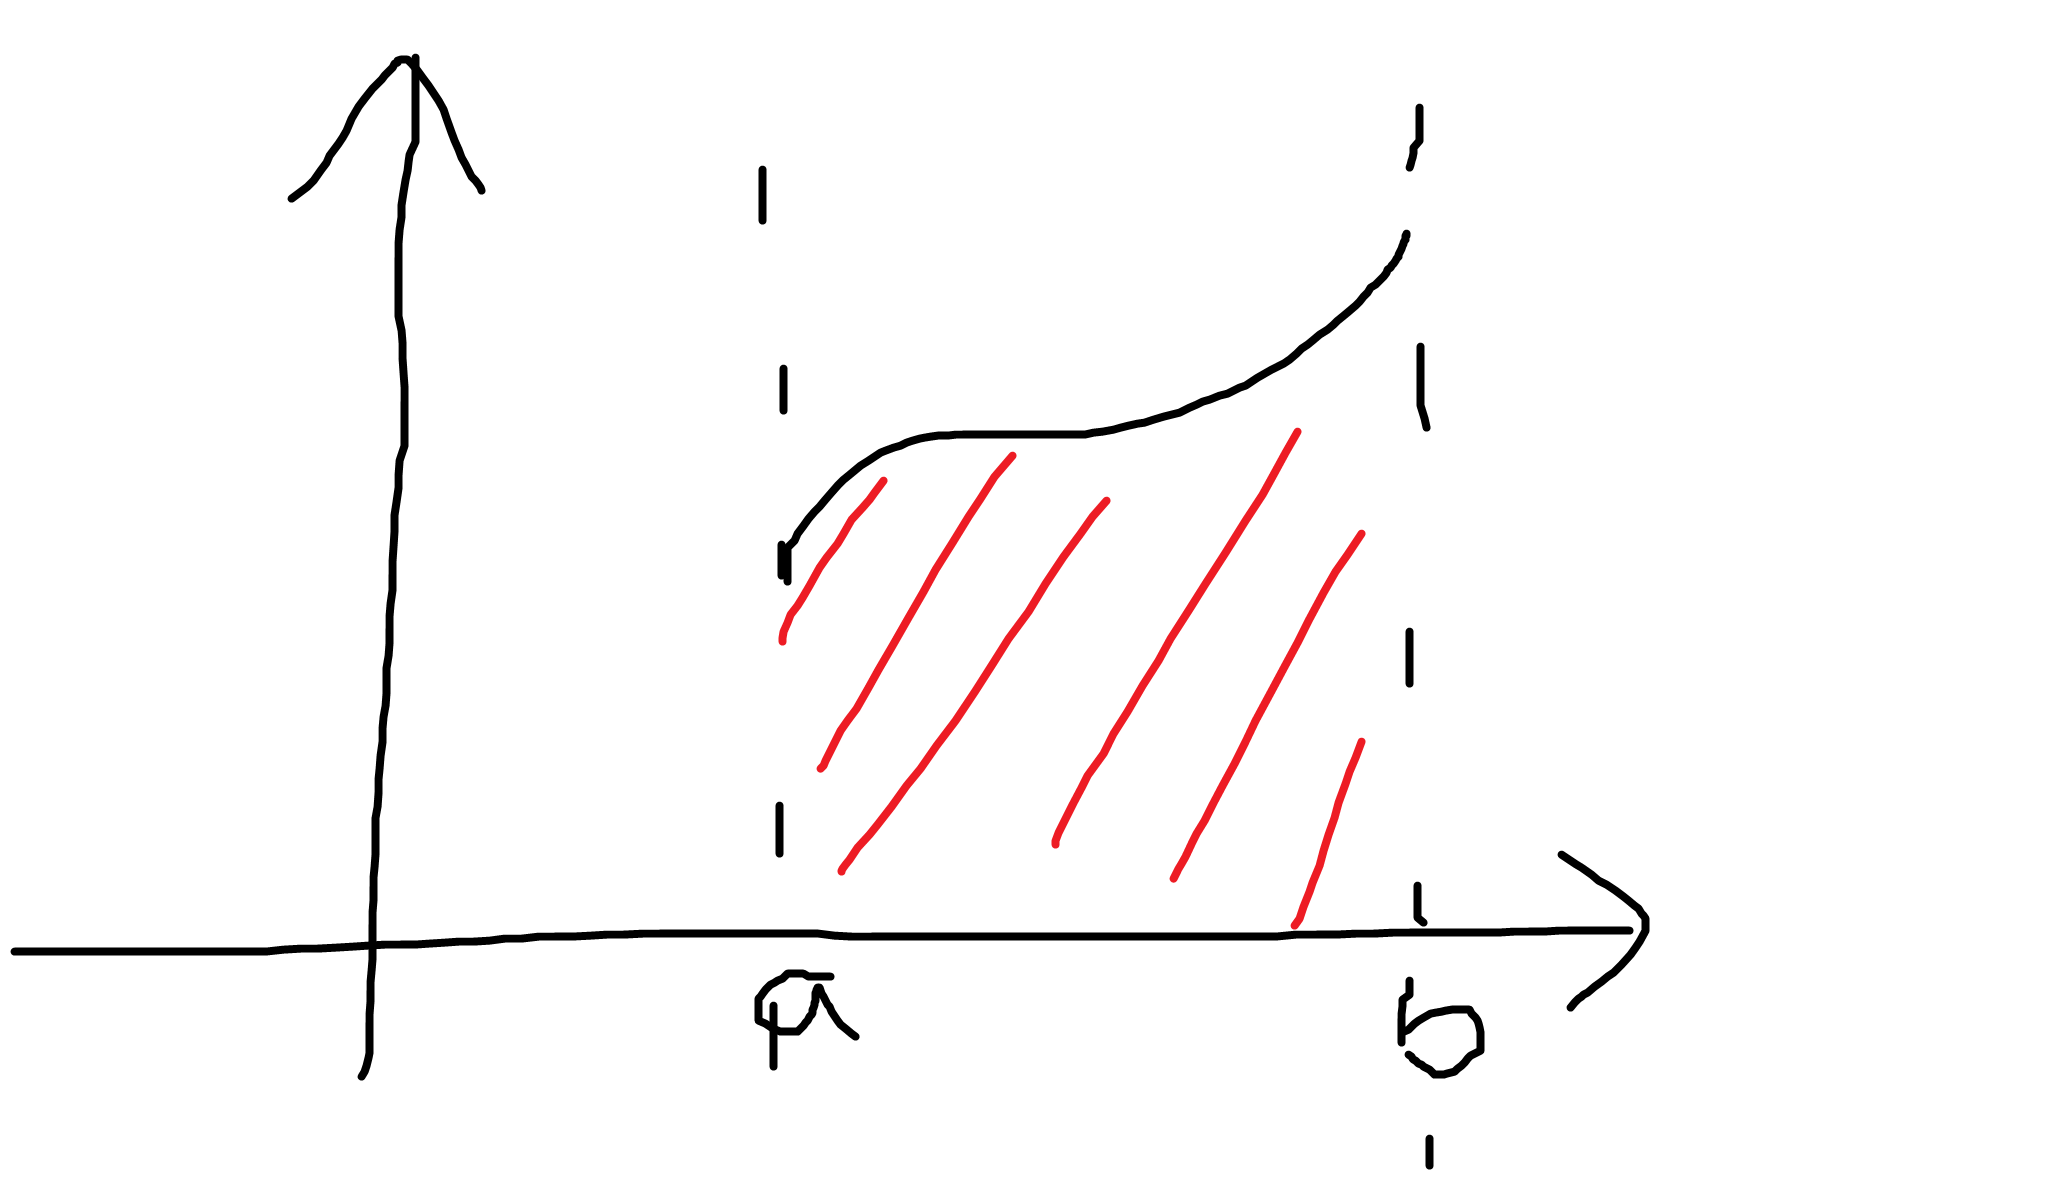
\includegraphics[height=3cm]{kepek/01.png}
			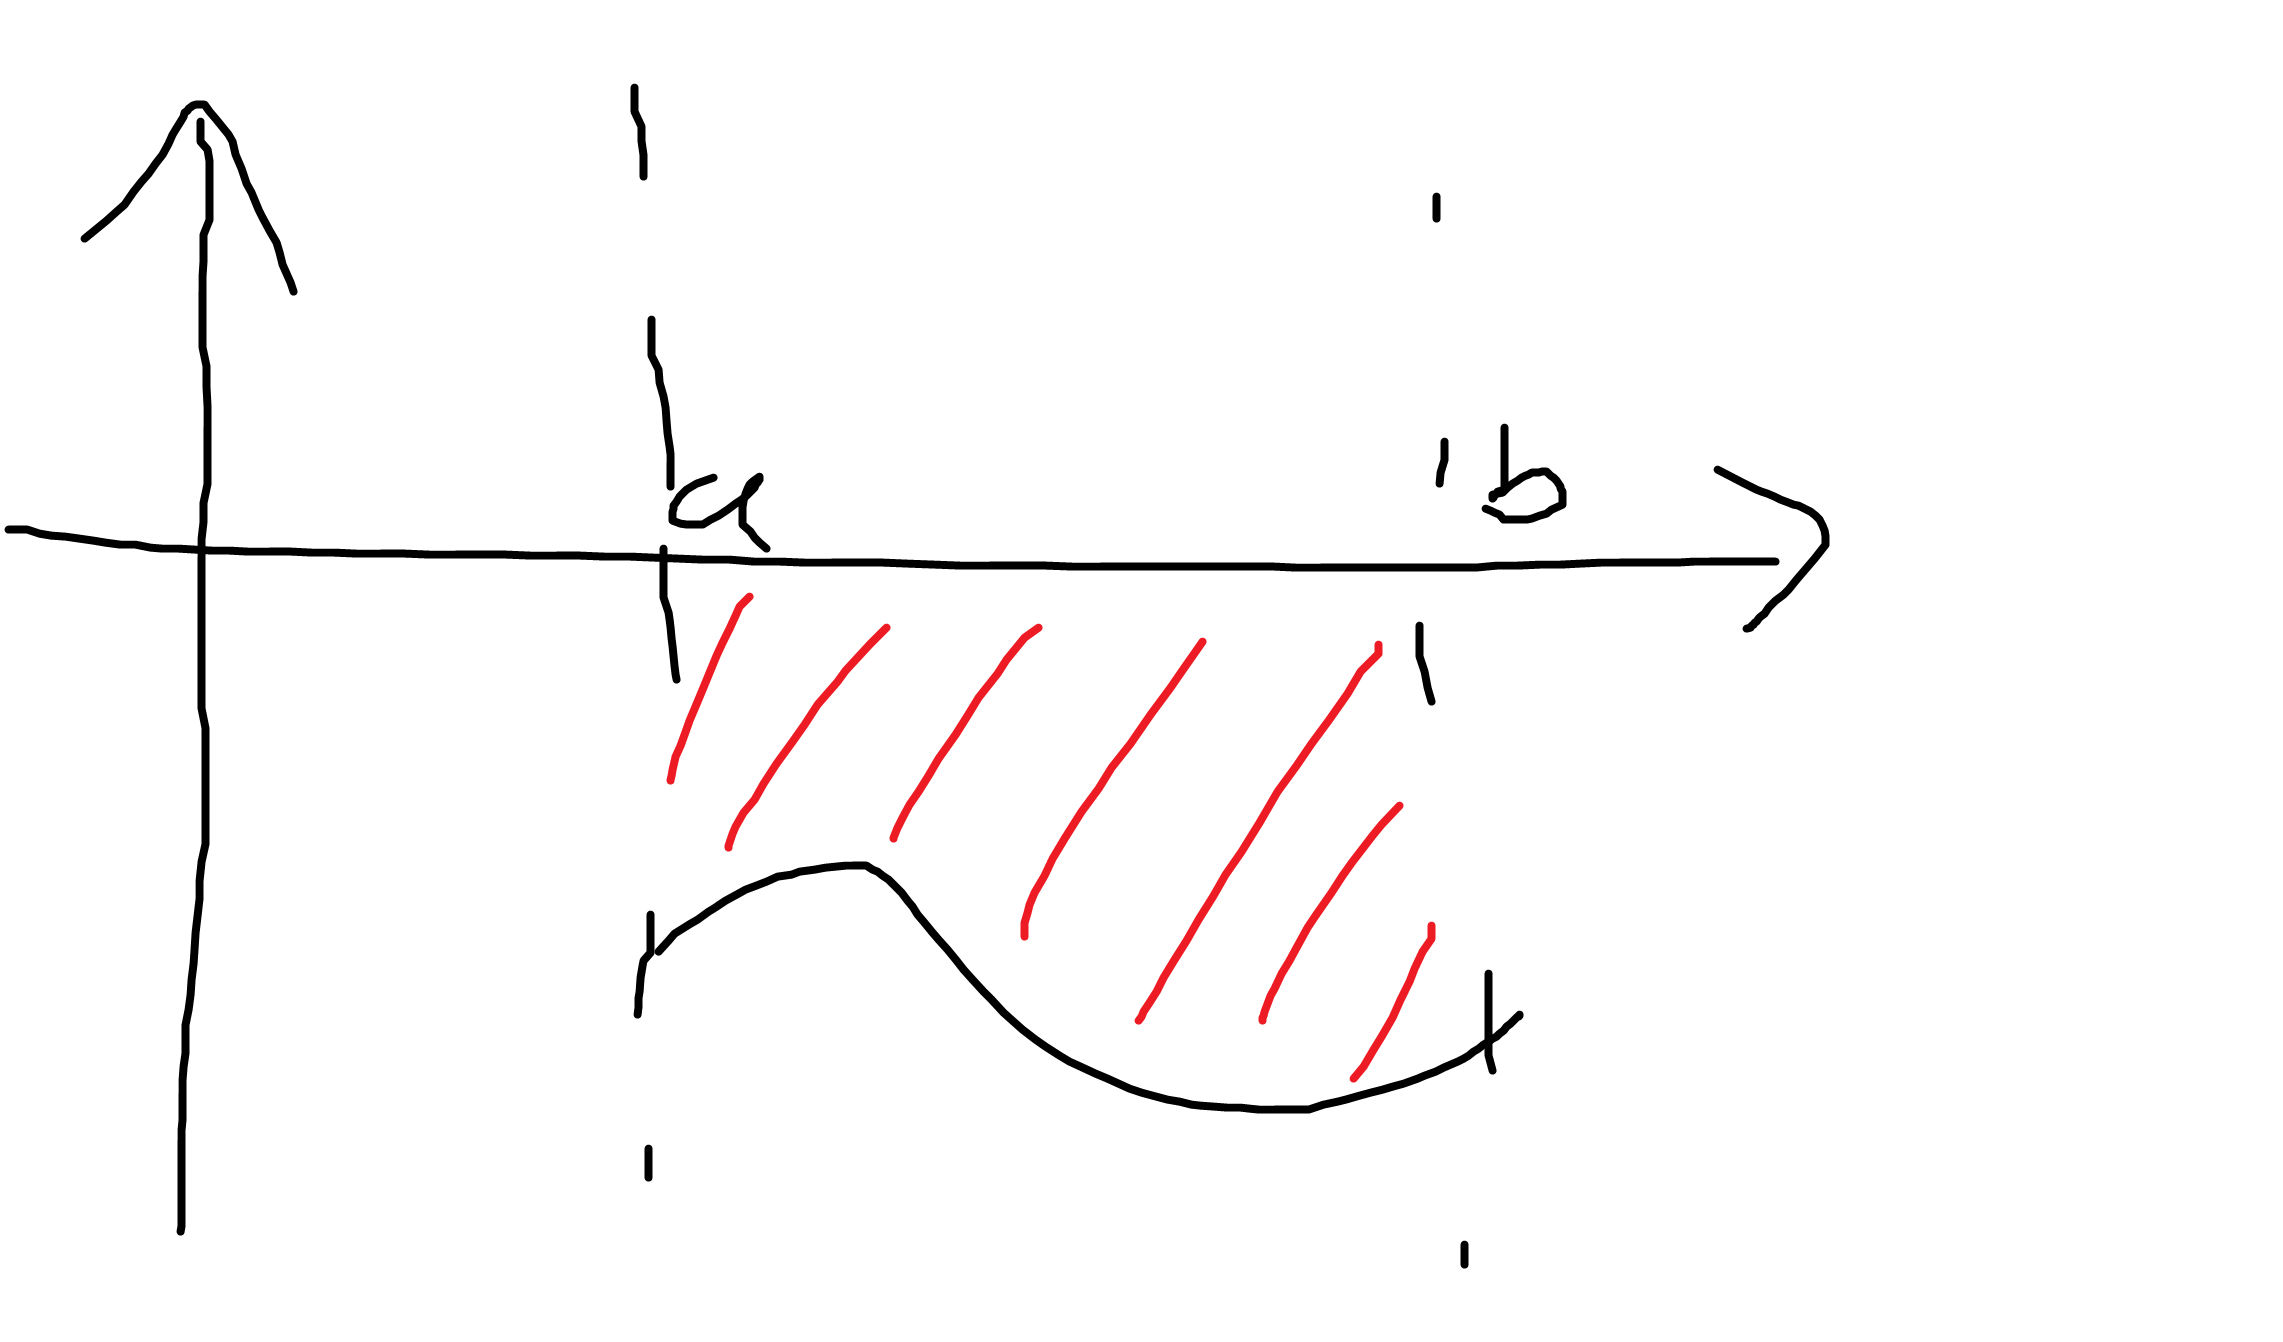
\includegraphics[height=3cm]{kepek/02.png}
			\caption{Rendre: $T=\int_a^bf,\quad f>0$,\quad valamint\quad  $T=\int_a^bf,\quad f<0$}
		\end{figure}
		\begin{figure}[H]
			\centering
			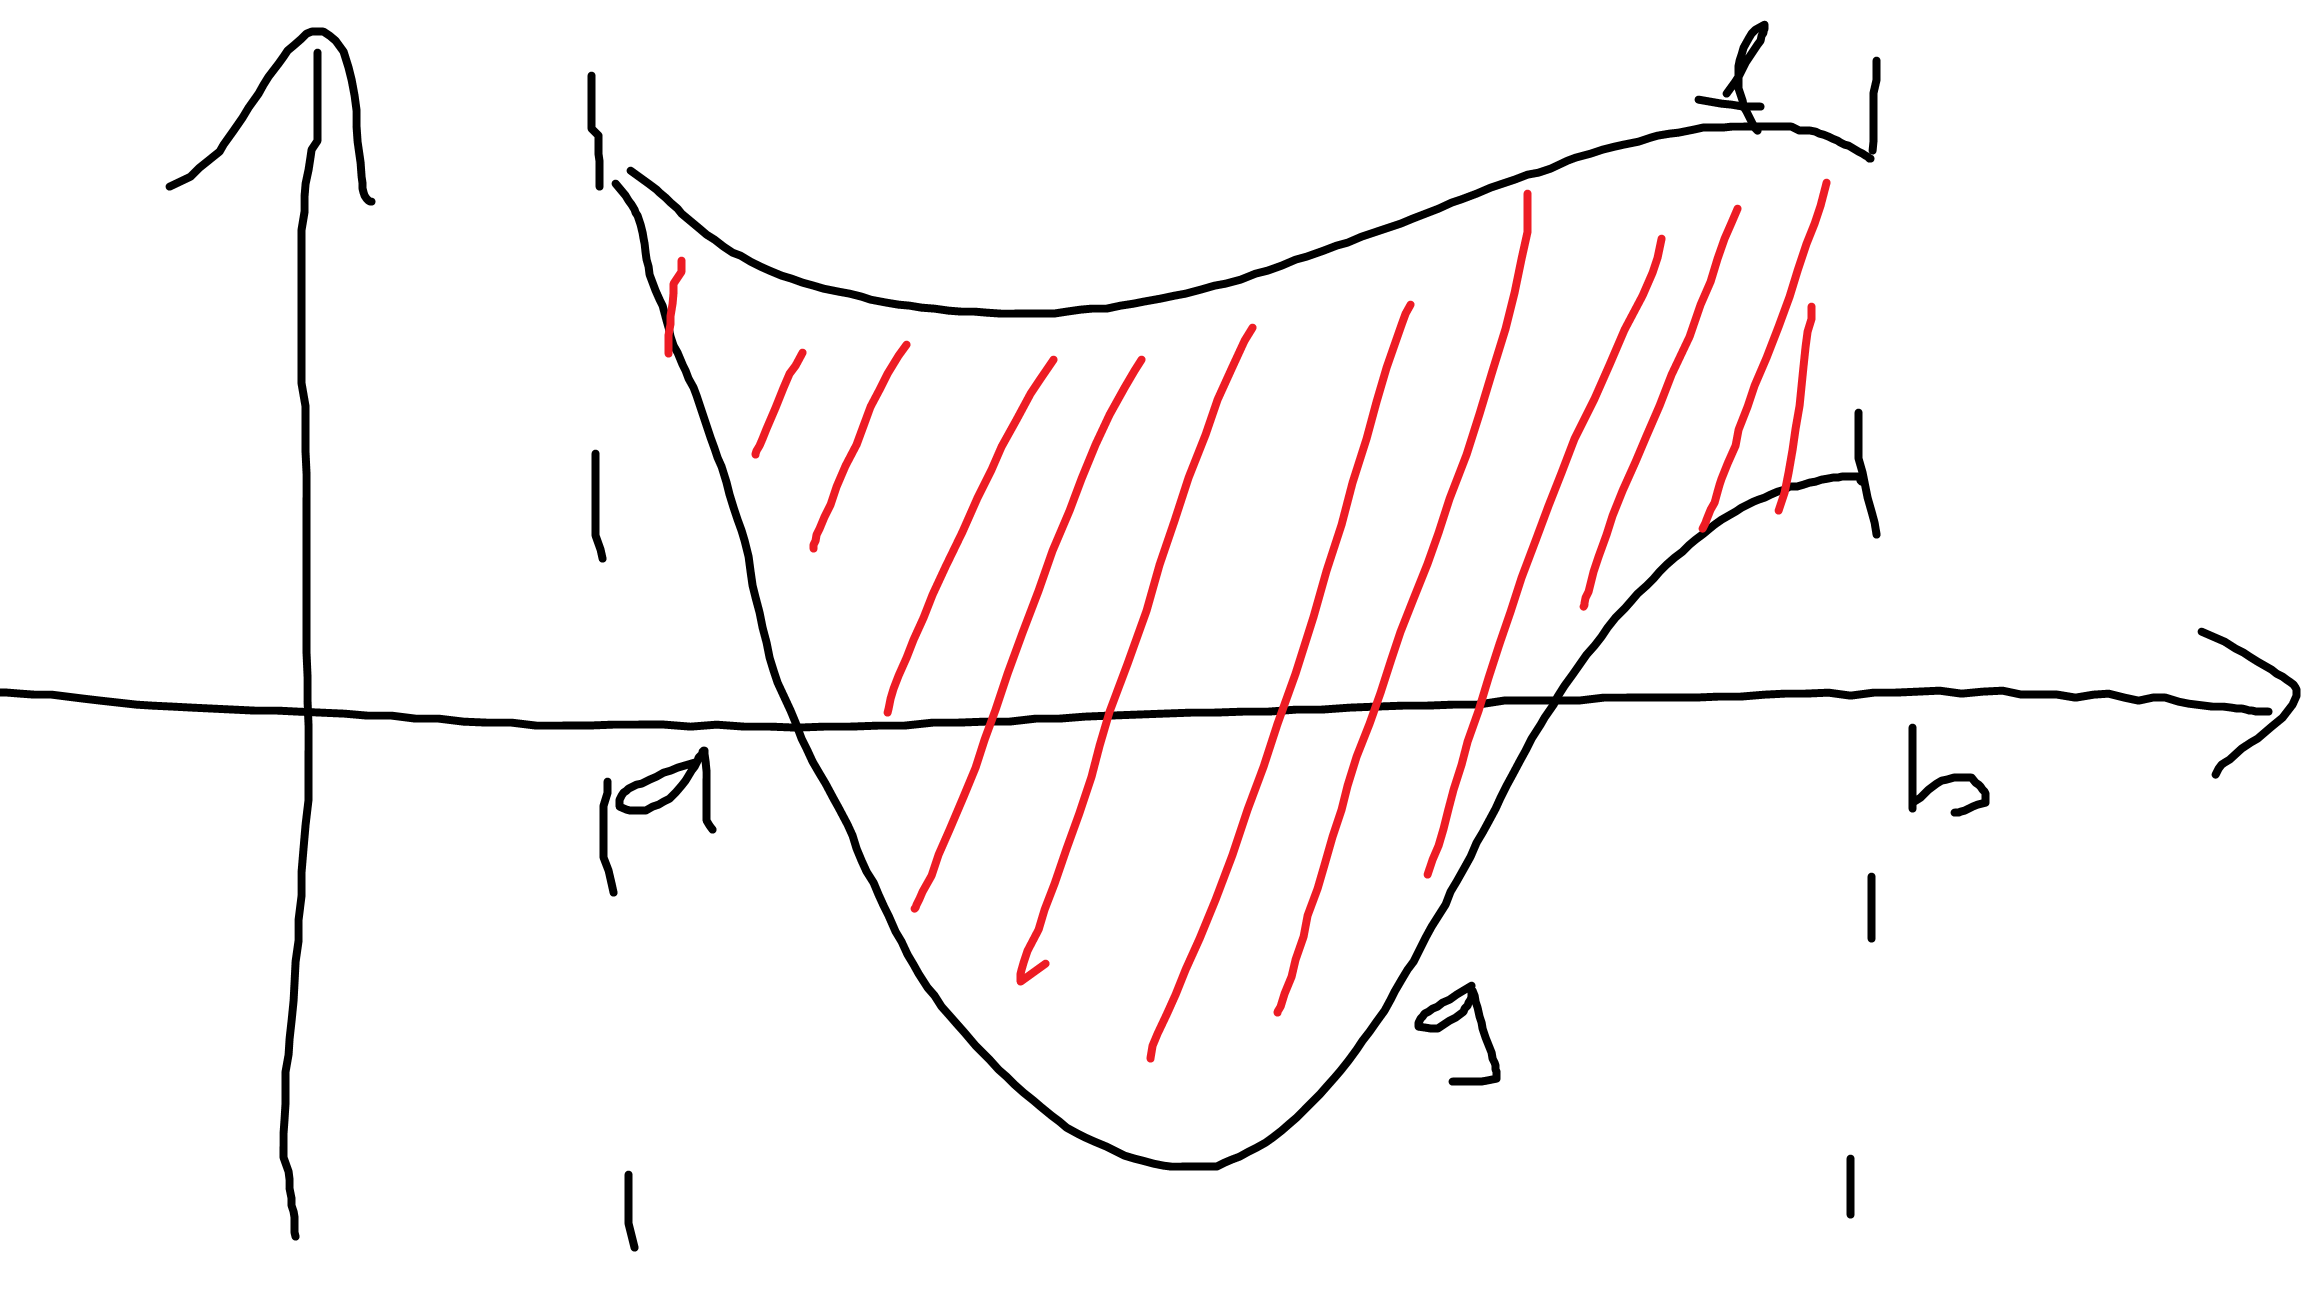
\includegraphics[height=3cm]{kepek/03.png}
			\caption{}\label{eltolatlan-fv}
		\end{figure}
		Hogyan lehet megoldani ezt? Megoldás: eltoljuk a függvényt.
		\begin{figure}[H]
			\centering
			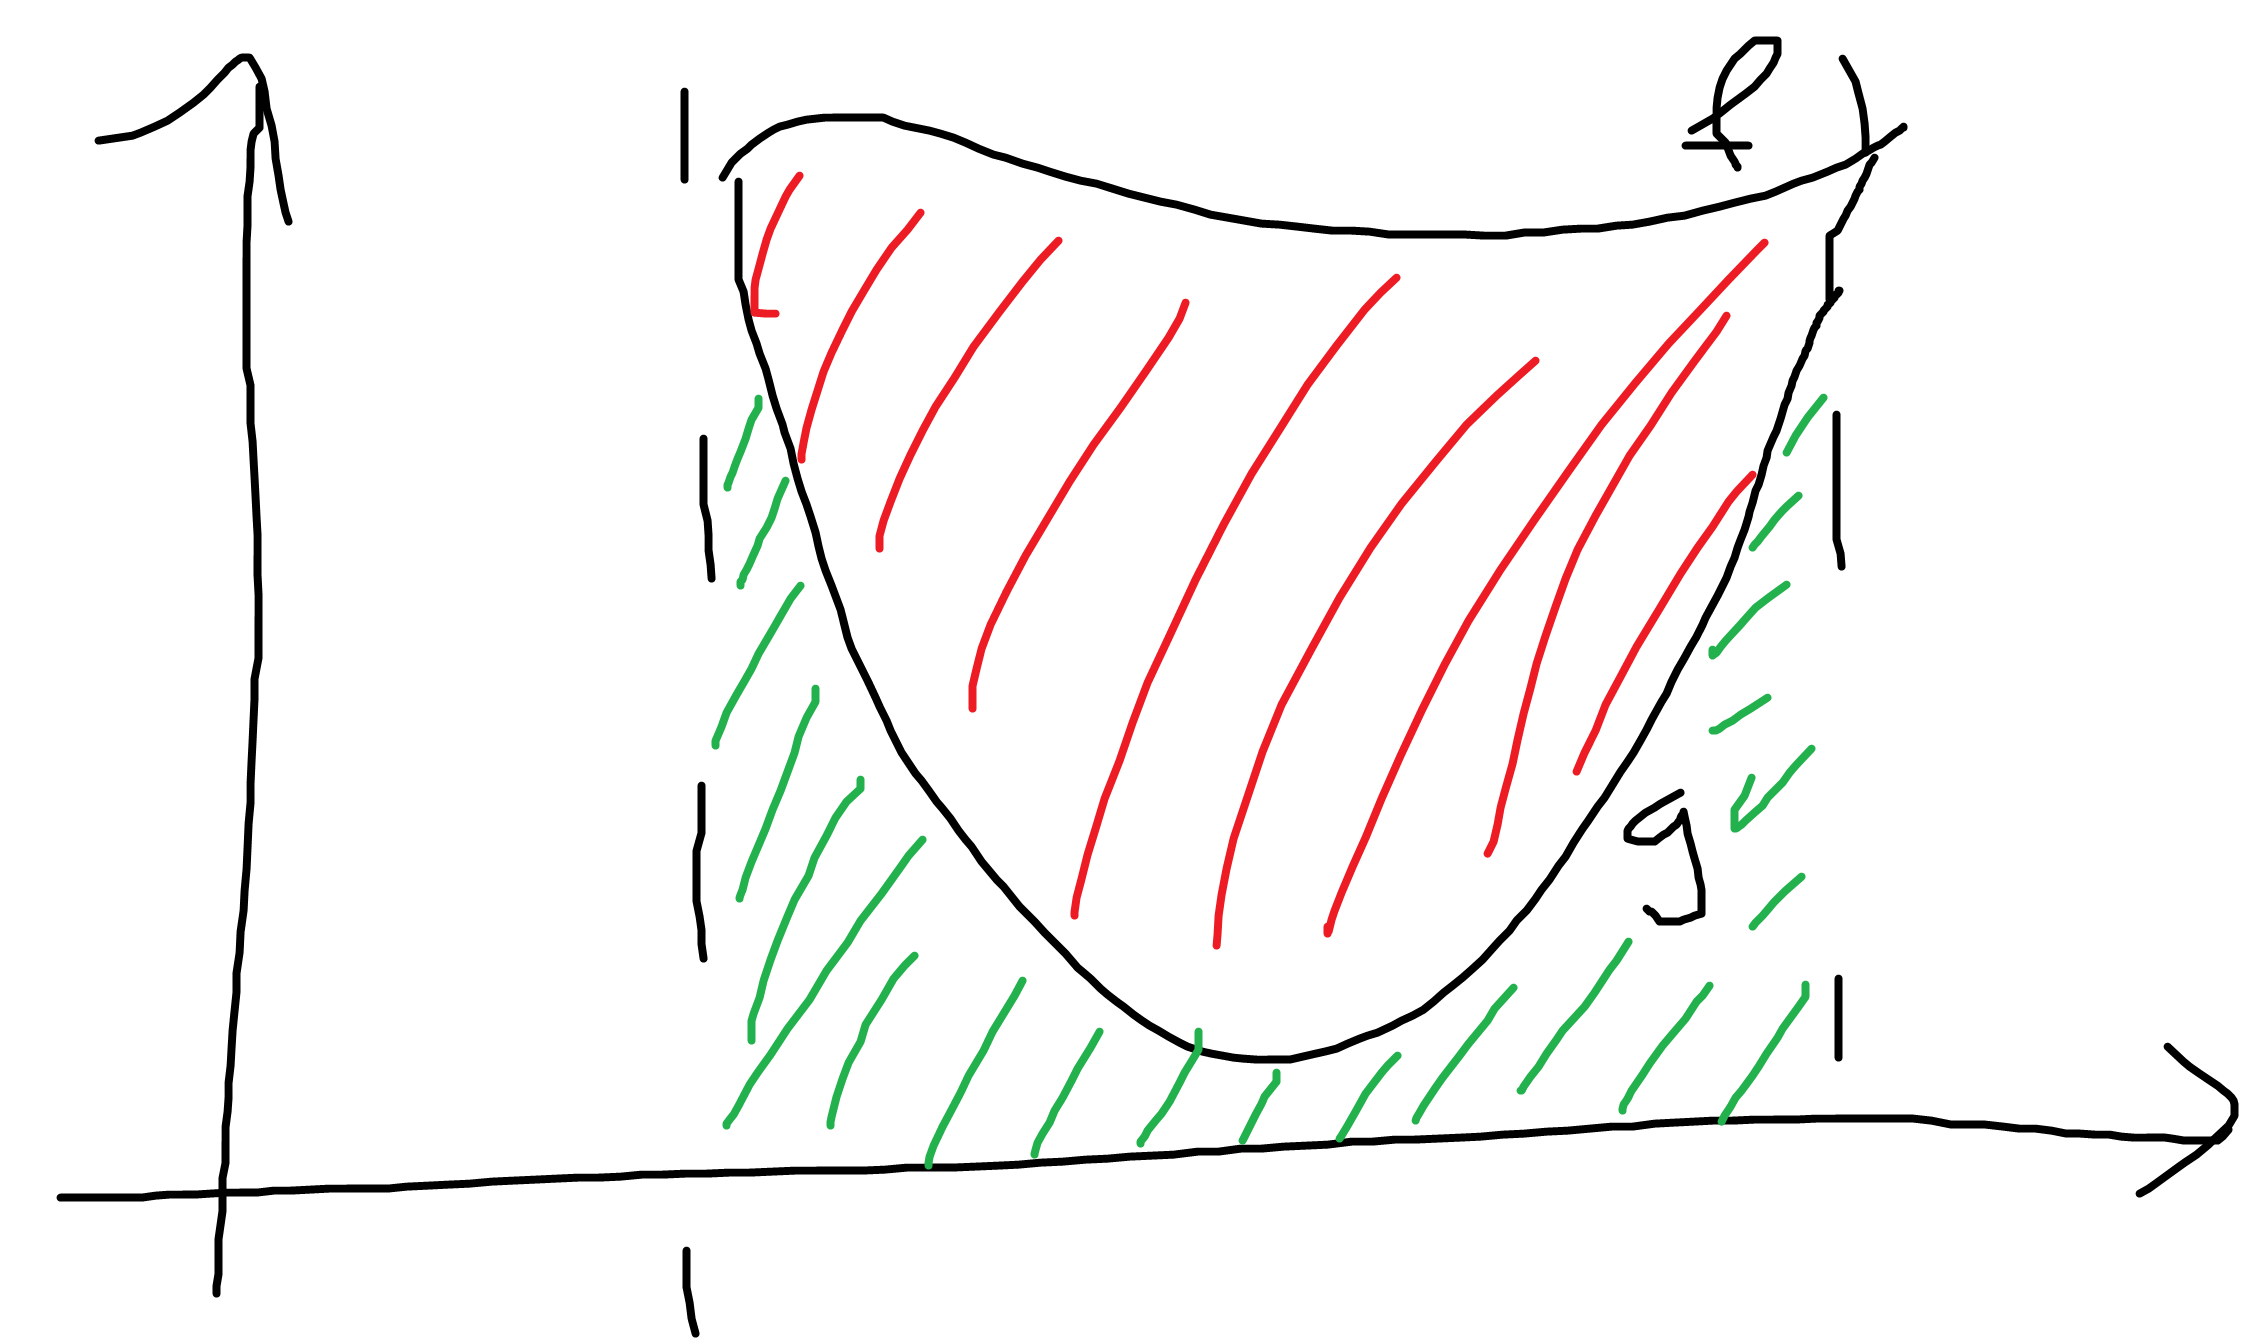
\includegraphics[height=2cm]{kepek/04.png}
			\caption{Ugyanaz az mint a \ref{eltolatlan-fv}. ábra, adott $c$ konstanssal eltolva.}
		\end{figure}
		Így már a terület könnyen meghatározható:
		\[ T=\int_a^b(f+c)-\int_a^b(g+c)=\int_a^b(f-g) \]
		\begin{figure}[H]
			\centering
			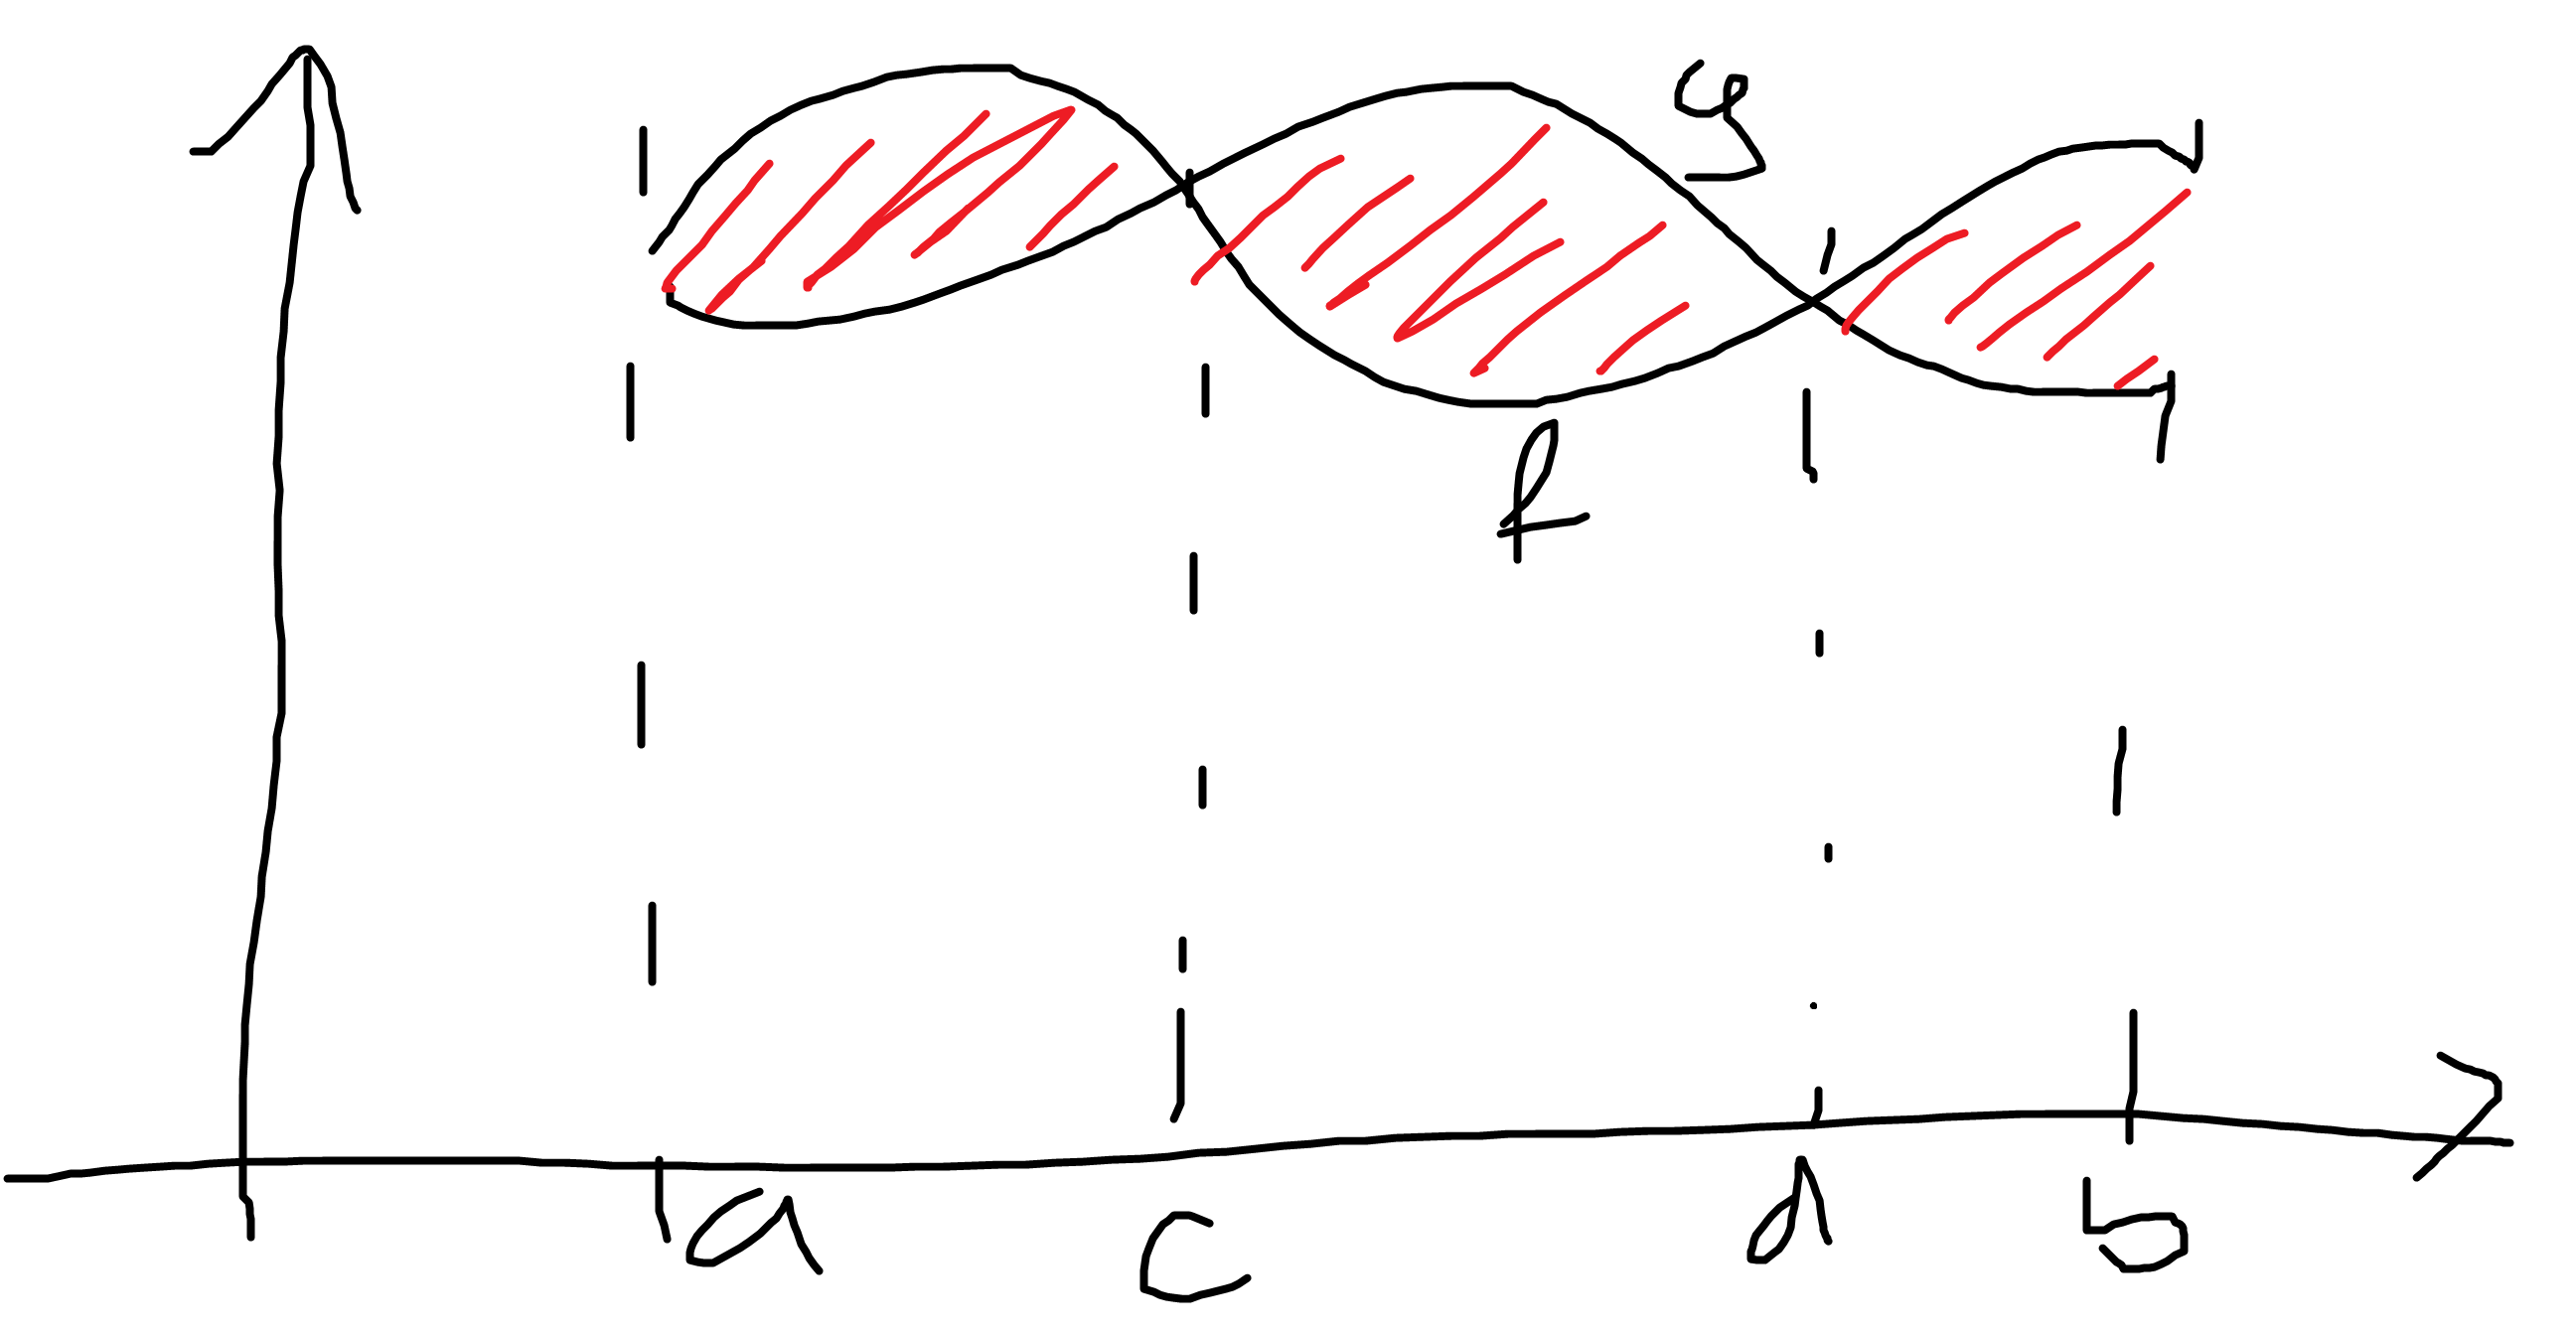
\includegraphics[height=3cm]{kepek/05.png}
			\caption{}
		\end{figure}
		\[ T=\int_a^c(f-g)+\int_c^d(g-f)+\int_d^b(f-g)=\int_a^b|f-g|= \]
		Megállapítható, hogy ez $f$ és $g$ 1-es metrikája.
		\[ =\rho_1(f,g),\quad (f,g\in C[a,b]) \]
		
		Szimmetriák kihasználása:
		\begin{figure}[H]
			\centering
			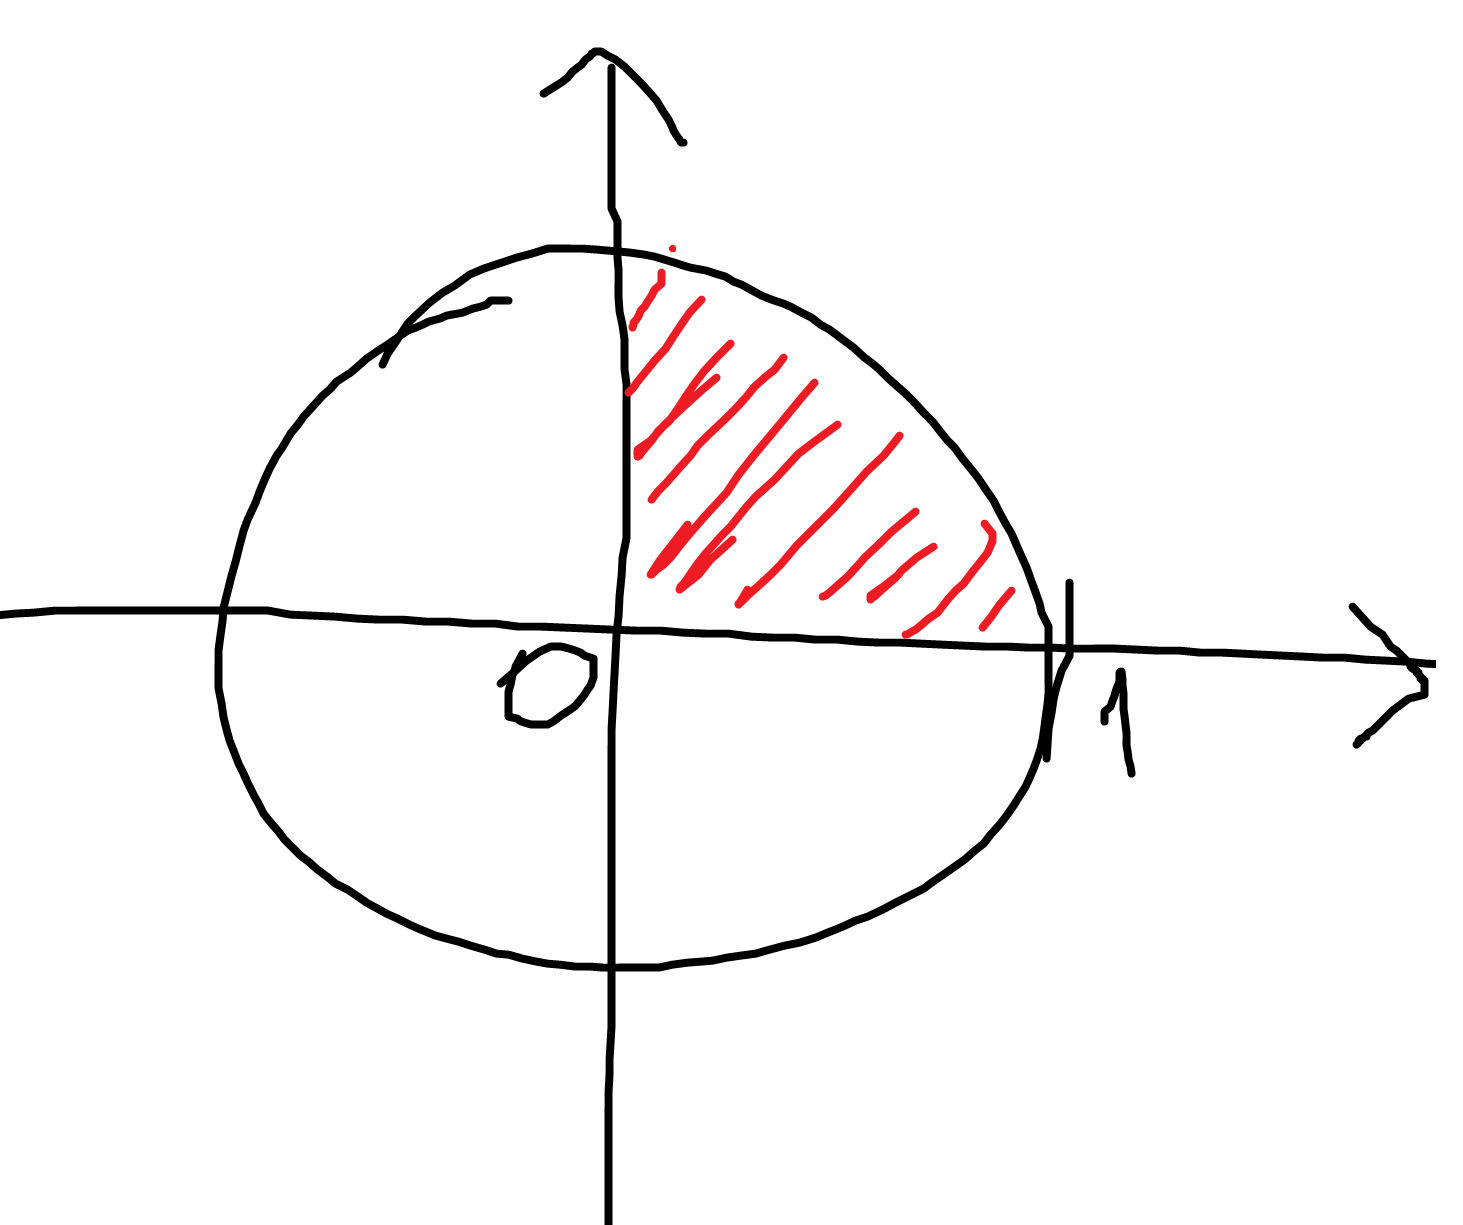
\includegraphics[height=3cm]{kepek/06.png}
			\caption{Elég a negyed kör területének meghatározása.}
		\end{figure}
		\[ T_{\text{kör}}=4\cdot T_{\text{negyedkör}}=4\cdot\int_0^1\sqrt{1-x^2}\,dx \]
		Szimmetria kihasználható így is:
		\begin{figure}[H]
			\centering
			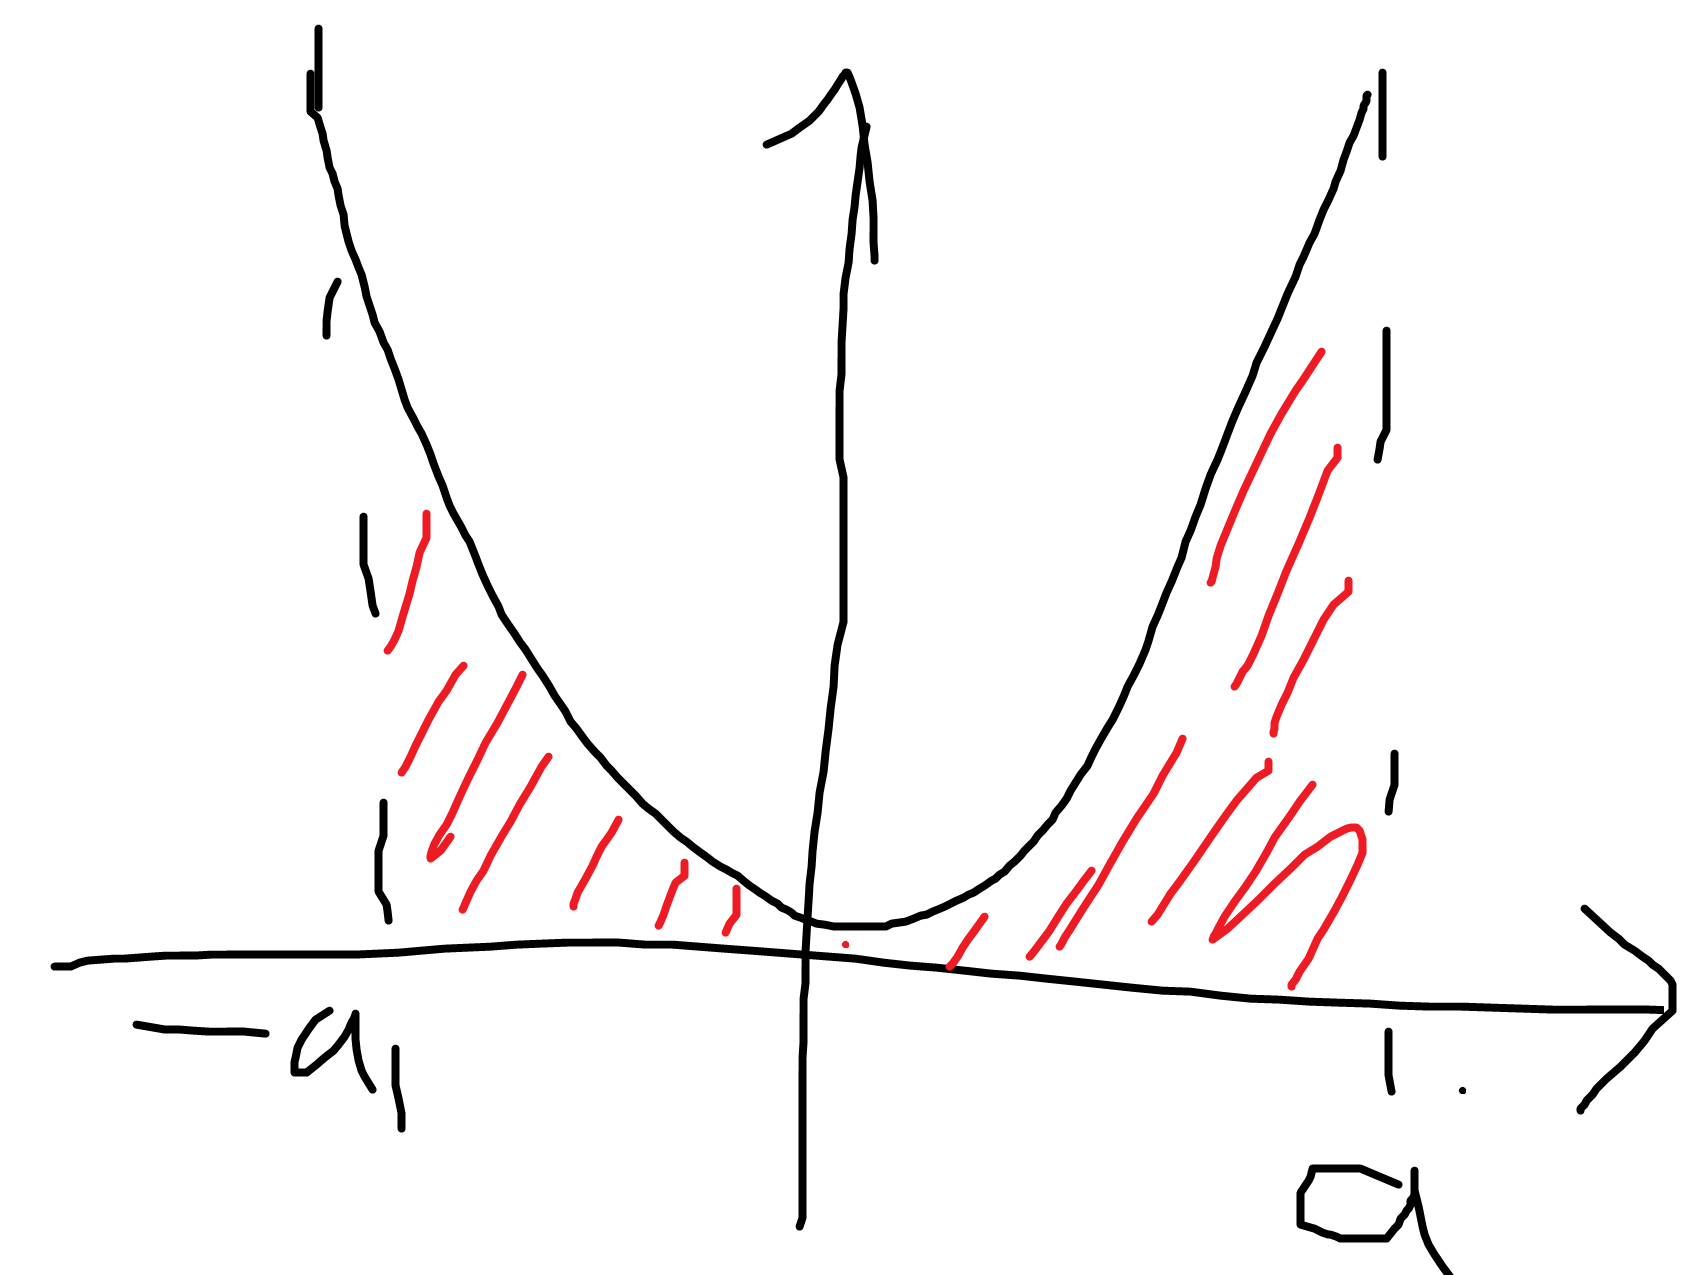
\includegraphics[height=3cm]{kepek/07.png}
			\caption{Elegendő a $[0,a]$ intervallumon a függvény integráltjának kétszeresét meghatározni.}
		\end{figure}
		\[ \int_{-a}^{a}f=2\cdot\int_0^af \]
		Megállapítható és kihasználható, hogy $f(x):=x^2$ páros.
		
		
	\begin{revision}
		Newton-Leibniz tétel: Ha $f\in\R[a,b]$ és $\int f\not=0$ 
			\[ \int_a^bf(x)\,dx=F(b)-F(a)=:[F(x)]_a^b\quad (\forall F\in\int f) \]
	\end{revision}
	\begin{example}
		Mennyi az e két \textit{reláció} által határolt terület?
			
		\[\begin{cases}
			y=x-1\\
			y^2=2x+6
		\end{cases}\]
		Világos, hogy a másik \textit{reláció} nem \textit{függvény}, azonban fel tudjuk írni két függvény együtteseként.
		\[y^2=2x+6\Leftrightarrow\quad y=\pm\sqrt{2x+6}\quad \Leftrightarrow\quad x=\frac{y^2-6}{2} \]
		\begin{figure}[H]
			\centering
			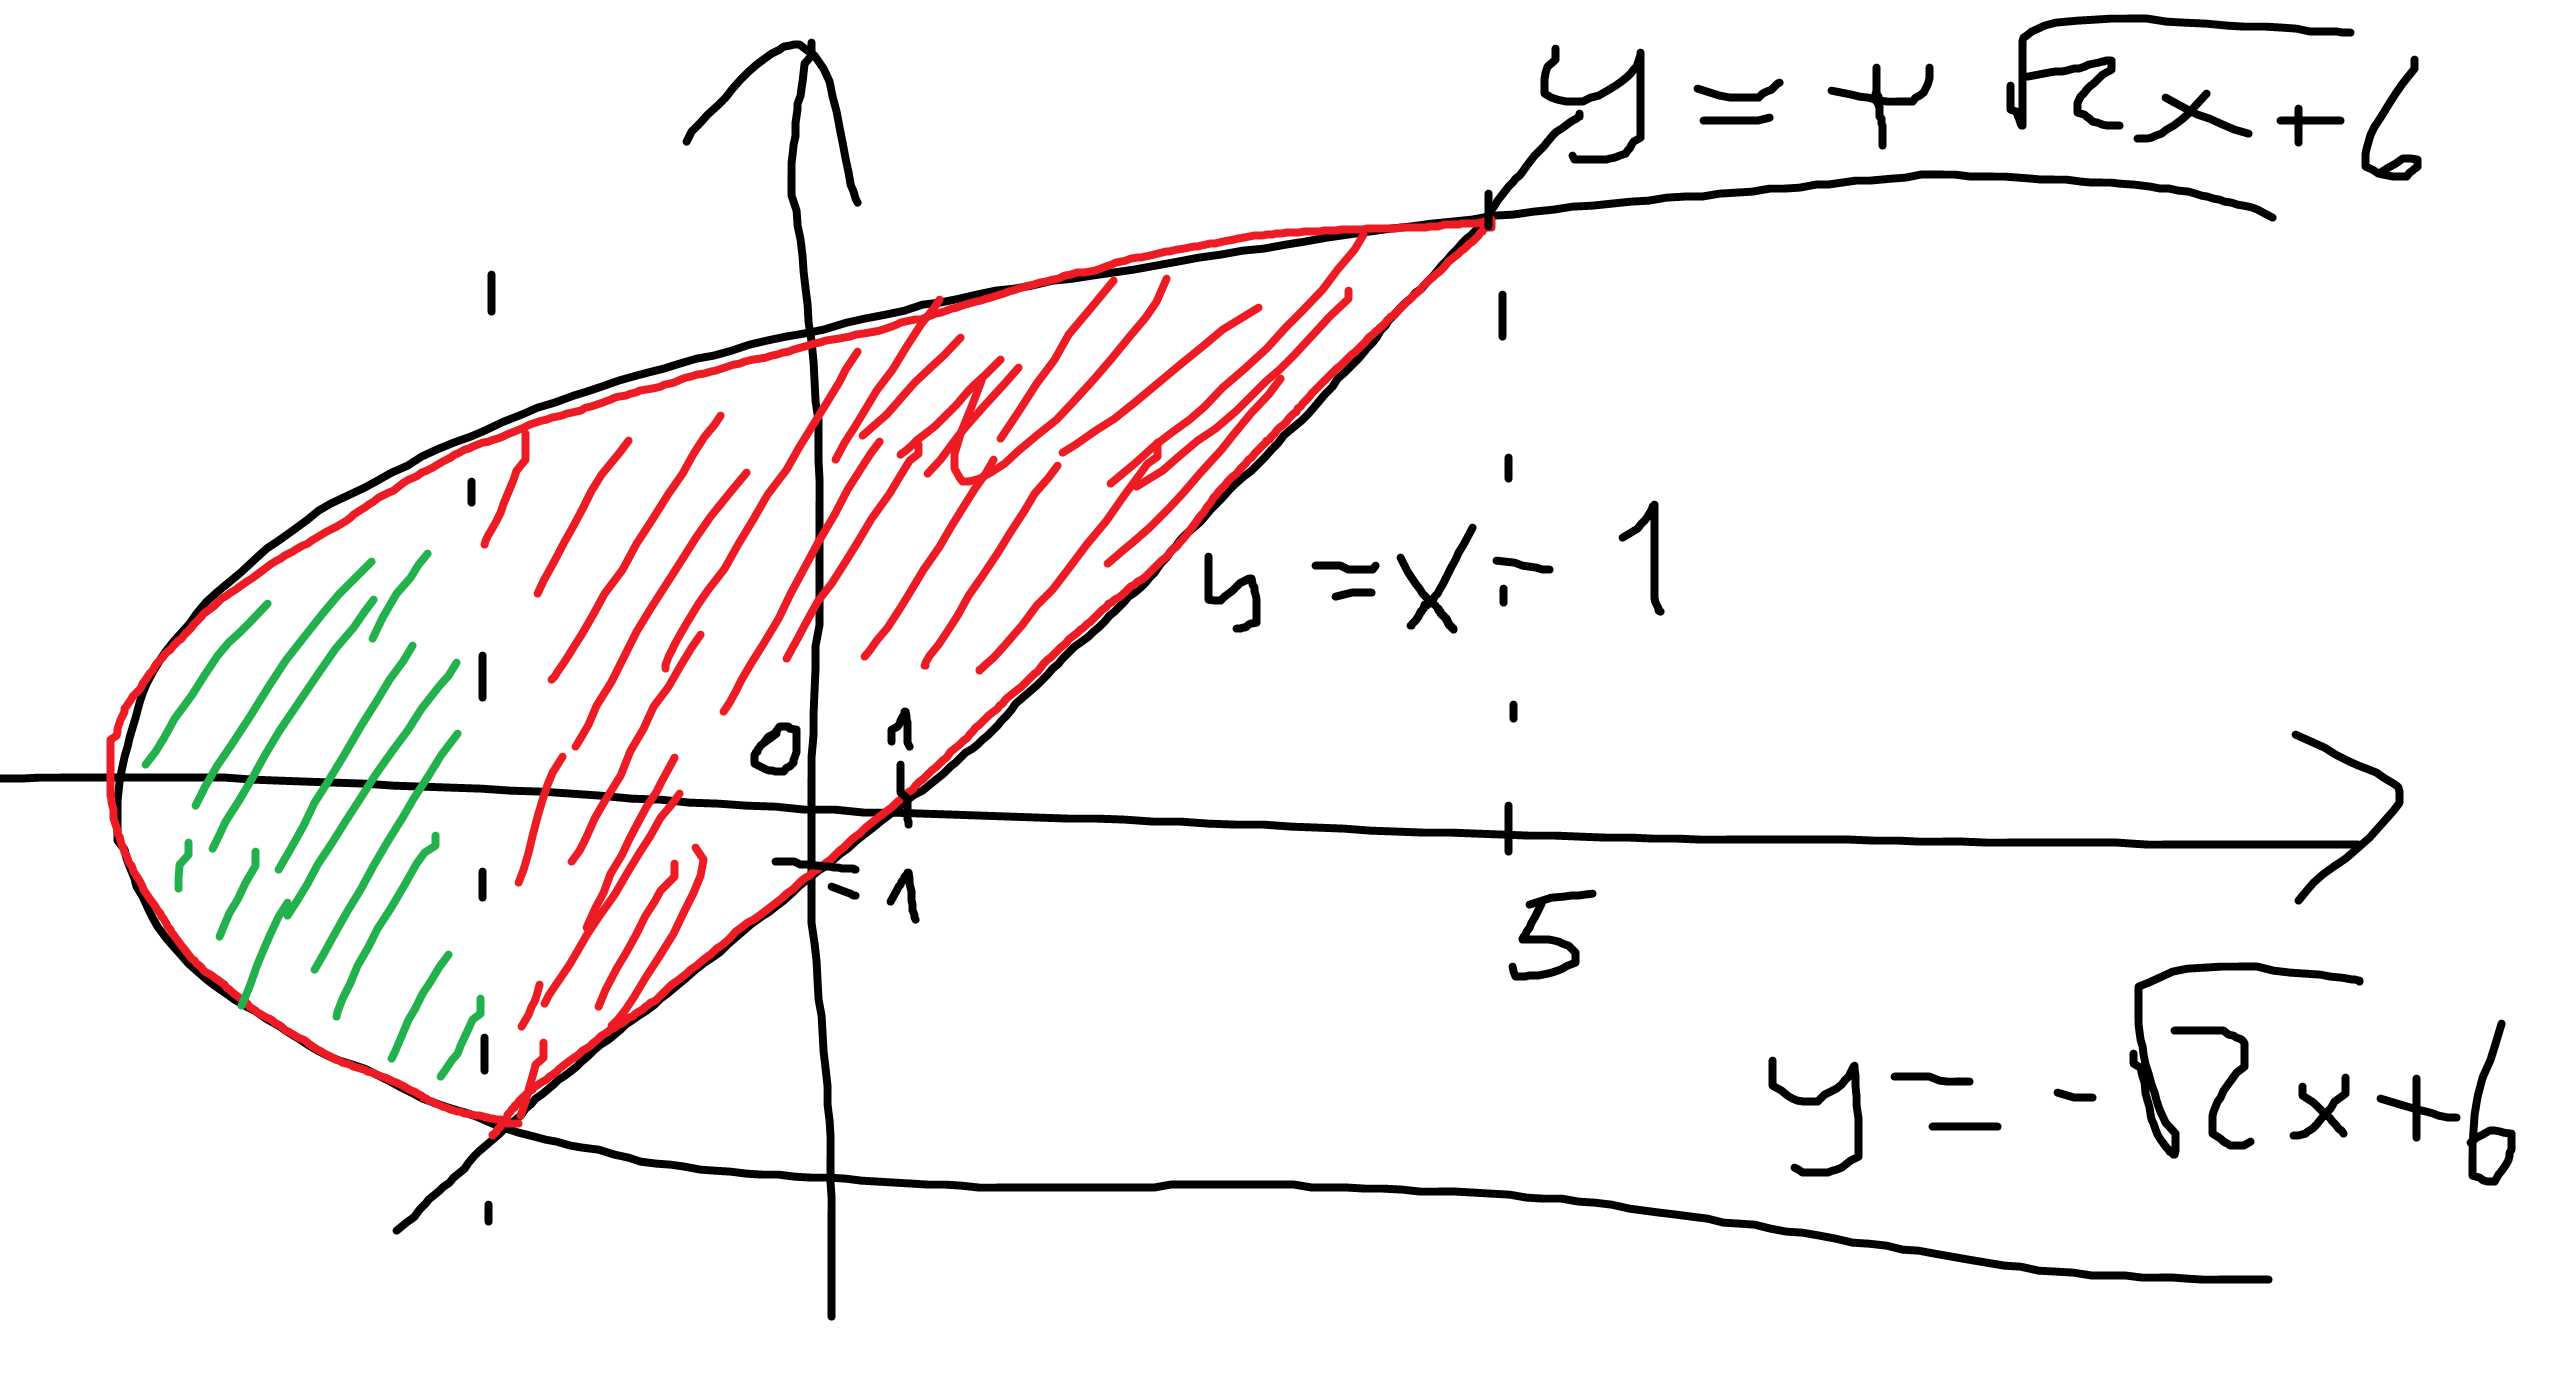
\includegraphics[height=3cm]{kepek/08.png}
			\caption{}
		\end{figure}
		Most már megállapítható a függvények metszéspontjai:
		\[ (x-1)^2=2x+6\quad \Leftrightarrow\quad x_1=-1\quad v.\quad x=5 \]
		Ez alapján a területet kiszámolhatjuk. A zöld területről megállapítható hogy szimmetrikus, és ezt ki is használhatjuk.
		\[ T=2\cdot\int_{-3}^{-1}\sqrt{2x+6}\,dx+\int_{-1}^{5}\left(\sqrt{2x+6}-(x-1)\right)\,dx=2\cdot\left[\frac{(2x+6)^{\frac{3}{2}}}{\frac{3}{2}\cdot2}\right]_{-3}^1+\left[\frac{(2x+6)^{\frac{3}{2}}}{\frac{3}{2}\cdot2}-\frac{x^2}{2}+x\right]_{5}^{-1}=\]
		\[=\frac{2}{3}\left[4^\frac{3}{2}-0\frac{3}{2}\right]+\frac{16^\frac{3}{2}}{3}-\frac{25}{2}+5-\left(\frac{4^\frac{3}{2}}{3}-\frac{1}{2}-1\right)=18  \]
	\end{example}
	\begin{example}Határozzuk meg az ezen görbék által határolt területet!
		\[\begin{cases}
			y=x^3\\
			y^2+x^2=2\\
			y=0
		\end{cases}\]
		\begin{figure}[H]
			\centering
			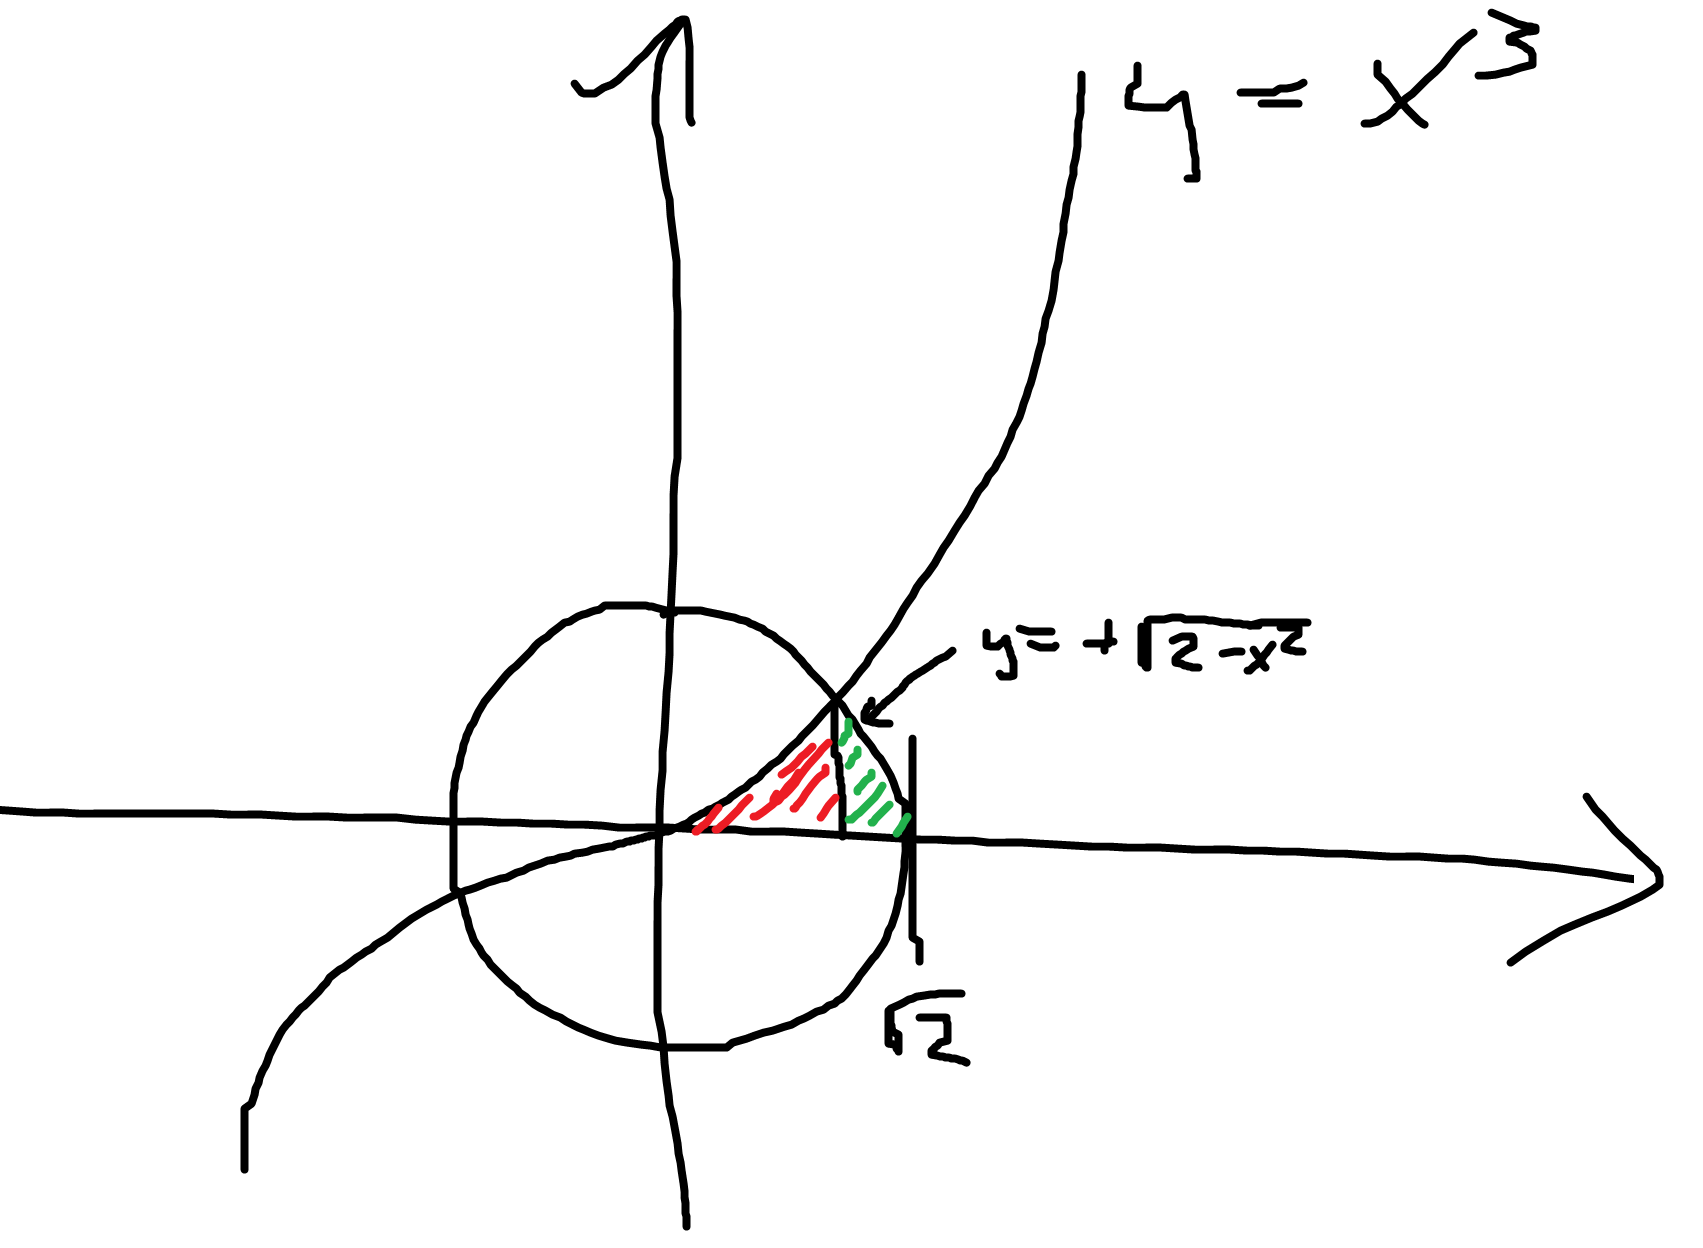
\includegraphics[height=4cm]{kepek/09.png}
			\caption{}
		\end{figure}
		Metszéspontok: (megfigyelhető, hogy az első egyenletet négyzetre emeltük)
		\begin{align*}
			x^2+x^6-2=0\\
			x^6-1+x^2-1=0\\
		\end{align*}
		Külön megállapítandó:
		\[(x^2-1)(x^4+x^2+1)=0\quad \Rightarrow\quad x=\pm1 \]
		\[ x^2-1=0\quad \Rightarrow\quad x=\pm1 \]
		Számoljuk ki  területet. A körre természetes okokból nem tudunk függvényt felírni, azonban megállapítható, hogy a számunkra fontos körnegyed egyenlete $y=+\sqrt{2-x^2}$.
		\[ T=\int_0^1x^3\,dx+\int_1^{\sqrt{2}}\sqrt{2-x^2}\,dx=\left[\frac{x^4}{4}\right]_0^1+I=\frac{1}{4}+I \]
		Ahol:
		\[ I=\int_1^{\sqrt{2}}\sqrt{2-x^2}\,dx=\sqrt{2}\cdot\int_1^{\sqrt{2}}\sqrt{1-\left(\frac{x}{\sqrt{2}}\right)^2}\,dx= \]
		Vezessünk be egy új változót.
		\[ \sin t:=\frac{x}{\sqrt{2}},\quad t=\arc\sin\left(\frac{x}{\sqrt{2}}\right) \]
		\[\text{Ha}\quad x=1\quad \Rightarrow\quad t=\arc\sin\frac{1}{\sqrt{2}}=\arc\sin\frac{\sqrt{2}}{2}=\frac{\pi}{4} \]
		\[\text{Ha}\quad x=\sqrt{2}\quad \Rightarrow\quad t=\arc\sin1=\frac{\pi}{2} \]
		Visszatérve:
		\[ =\sqrt{2}\cdot\int_{\frac{\pi}{4}}^{\frac{\pi}{2}}\sqrt{1-\sin^2t}\cdot\sqrt{2}\cos t\,dt= \]
		Visszahelyettesíteni fölösleges, hisz nem primitív függvényt, hanem egy konkrét számot keresünk.
		\[ =2\cdot\int_{\frac{\pi}{4}}^{\frac{\pi}{2}}|\cos t|\cdot\cos t\,dt\quad \overset{\frac{\pi}{4}\leq t\leq \frac{\pi}{2}}{=}\quad2\cdot\int_{\frac{\pi}{4}}^{\frac{\pi}{2}}\overbrace{\cos^2t}^{\frac{1+\cos2t}{2}}\,dt=\left[t+\frac{\sin2t}{2}\right]_{\frac{\pi}{4}}^{\frac{\pi}{2}}=\frac{\pi}{2}+\frac{\sin\pi}{2}-\frac{\pi}{4}-\frac{\sin\frac{\pi}{2}}{2}=\frac{\pi}{4}-\frac{1}{2}  \]
	\end{example}
	\begin{note}
		Okkal $I$-vel, és nem $I(x)$-el jelölünk. A határozatlan integrál egy függvény, a határozott csupán egy szám.
	\end{note}
	\begin{example}
		Számítsuk ki a következő minimumot:
		\[ \min\left\{\int _0^1|x^2-c|\,dx\quad :\quad c\in\R \right\} \]
		\begin{figure}[H]
			\centering
			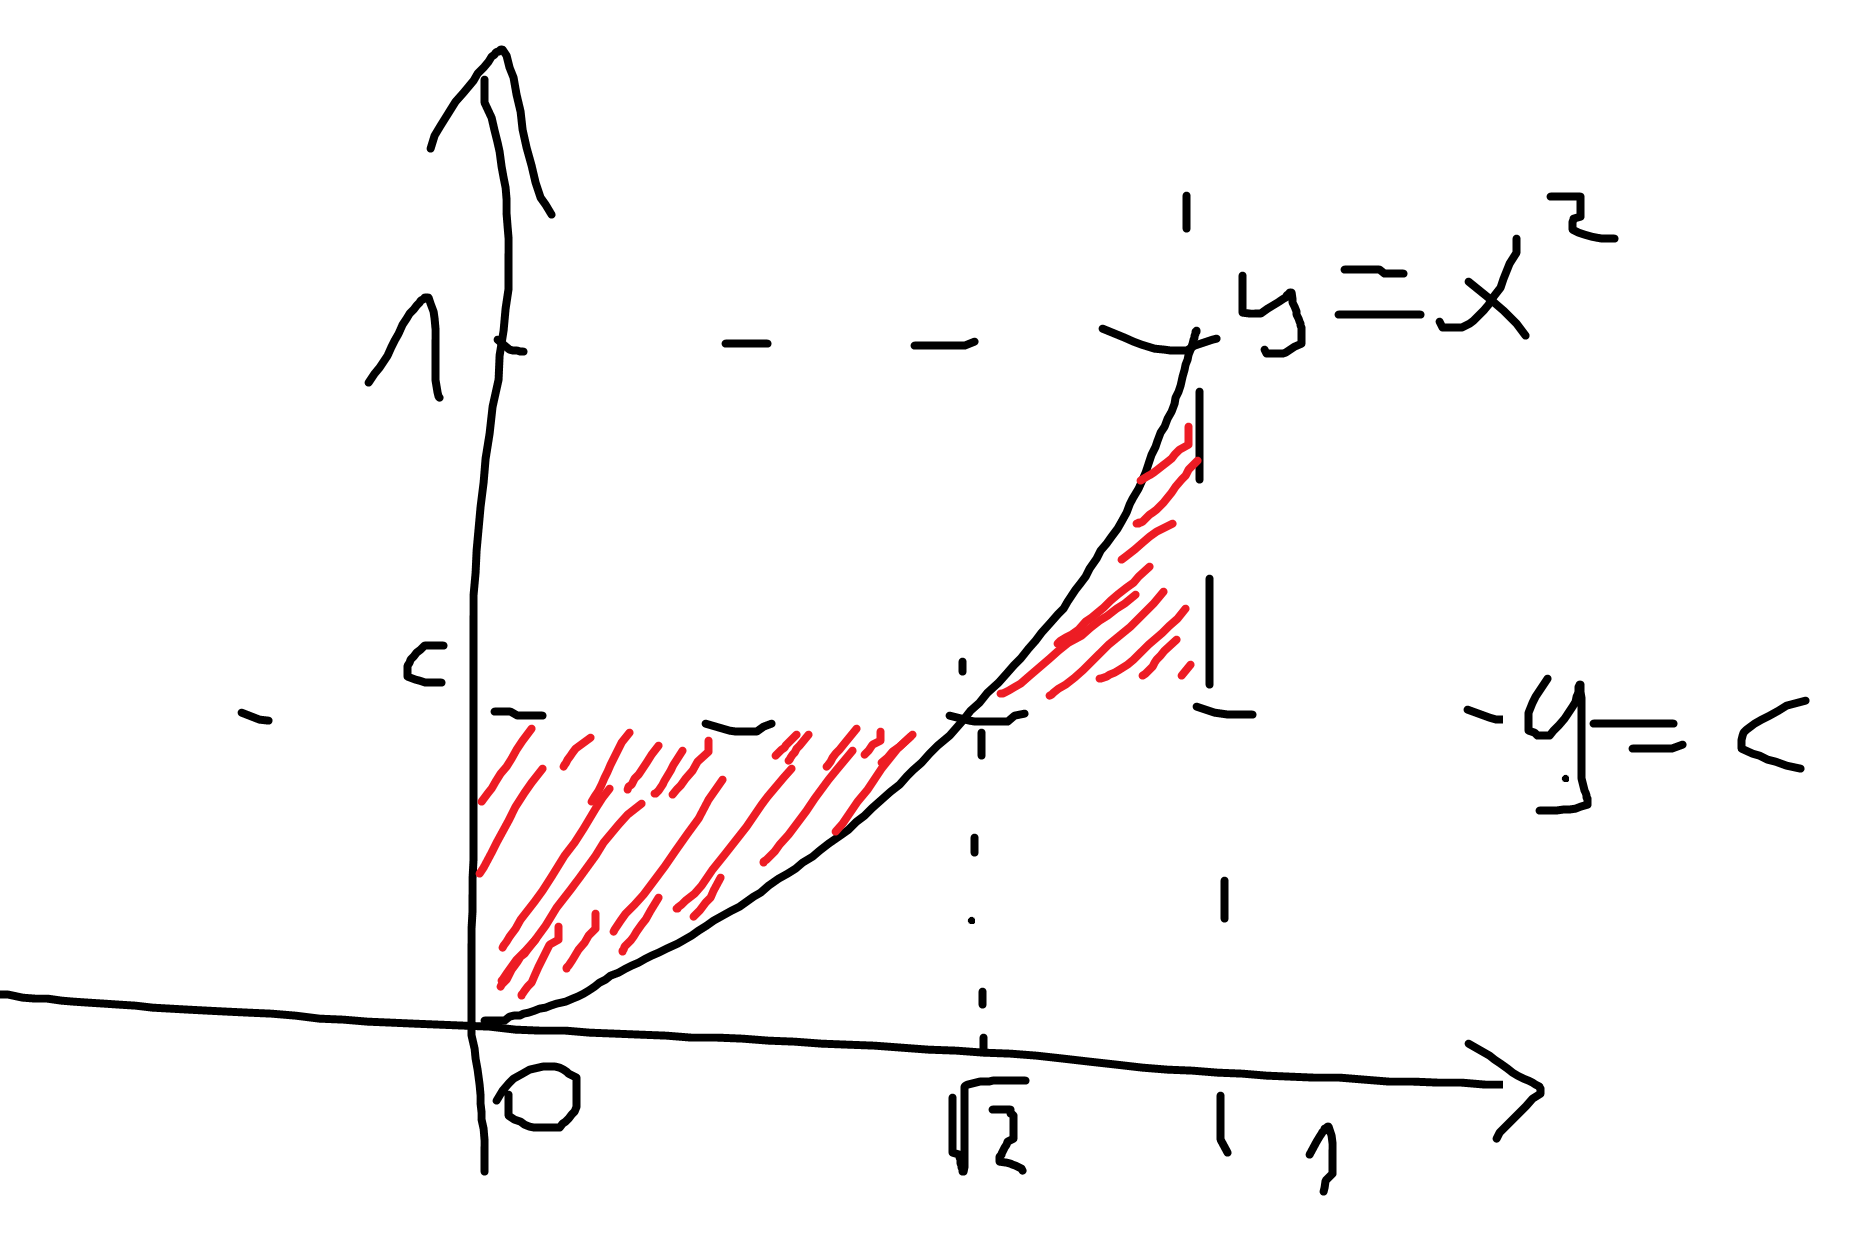
\includegraphics[height=3cm]{kepek/10.png}
			\caption{}
		\end{figure}
		
		Azaz, hogyan kell meghúzni az egyenest úgy, hogy a terület a legkisebb legyen? Világos, hogy elég $c\in[0,1]$ intervallumot vizsgálnunk, ui. ellenkező esetben 1-1 téglalap területével nő a terület.
		\smallskip
		
		Metszéspontok:
		\[ x^2=x\quad \Leftrightarrow\quad x=\pm\sqrt{c}\quad \Rightarrow\quad x=\sqrt{c}\in[0,1] \]
		Határozzuk meg a területet:
		\[ T(c)=\int_0^{\sqrt{c}}(c-x^2)\,dx+\int_{\sqrt{c}}^{1}(x^2-c)\,dx=\left[cx-\frac{x^3}{3}\right]_0^{\sqrt{c}}+\left[\frac{x^3}{3}-cx\right]^1_{\sqrt{c}}=c\sqrt{c}-\frac{c\sqrt{c}}{3}+\frac{1}{3}-c-\frac{c\sqrt{c}}{3}+c\sqrt{c}=\]
		\[=\frac{4}{3}c\sqrt{c}-c+\frac{1}{3}\quad c\in[0,1] \]
		Kompakt halmazon folytonos függvényt vizsgálunk, és kell hogy legyen maximum vagy minimum. Ez lehet 0 vagy 1, vagy intervallumon belül. Ha $c\in(0,1)$ akkor:
		\[T'(c)=\frac{4}{3}\cdot\frac{3}{2}\cdot\sqrt{c}-1=2\cdot\sqrt{c}-1=0\quad \Leftrightarrow\quad c=\frac{1}{4}\in(0,1)\checkmark \]
		\begin{center}		
			\begin{tabular}{l|c|c|c}
				$T'(x)$&$-$&0&$+$\\
				\hline
				$T(x)$&$\frac{1}{3}\searrow$&$\frac{1}{4}$&$\nearrow\frac{2}{3}$
			\end{tabular}
		\end{center}
		\[ T(0)=\frac{1}{3};\quad T(1)=\frac{2}{3};\quad T\left(\frac{1}{4}\right)=\frac{1}{4} \]
		Összefoglalva, a terület minimális a $c=\frac{1}{4}$ választással.
	\end{example}
	\begin{note}
		Mi ez a feladat? $f(x):=x^2, \quad x\in[0,1];\quad g(x):=c;\quad \rho_1(f,g):=\int_0^1|f-g|$
		\[ \Rightarrow\quad (C[0,1];\rho_1) \quad \text{m. tér};\quad \min\left\{\rho_1(f,g)\ | \ y=c\in\R\right\} \]
	\end{note}
	\subsubsection{Ívhossz számolás}
	\begin{note}
		$f\in C^1[a,b]$
		\begin{figure}[H]
			\centering
			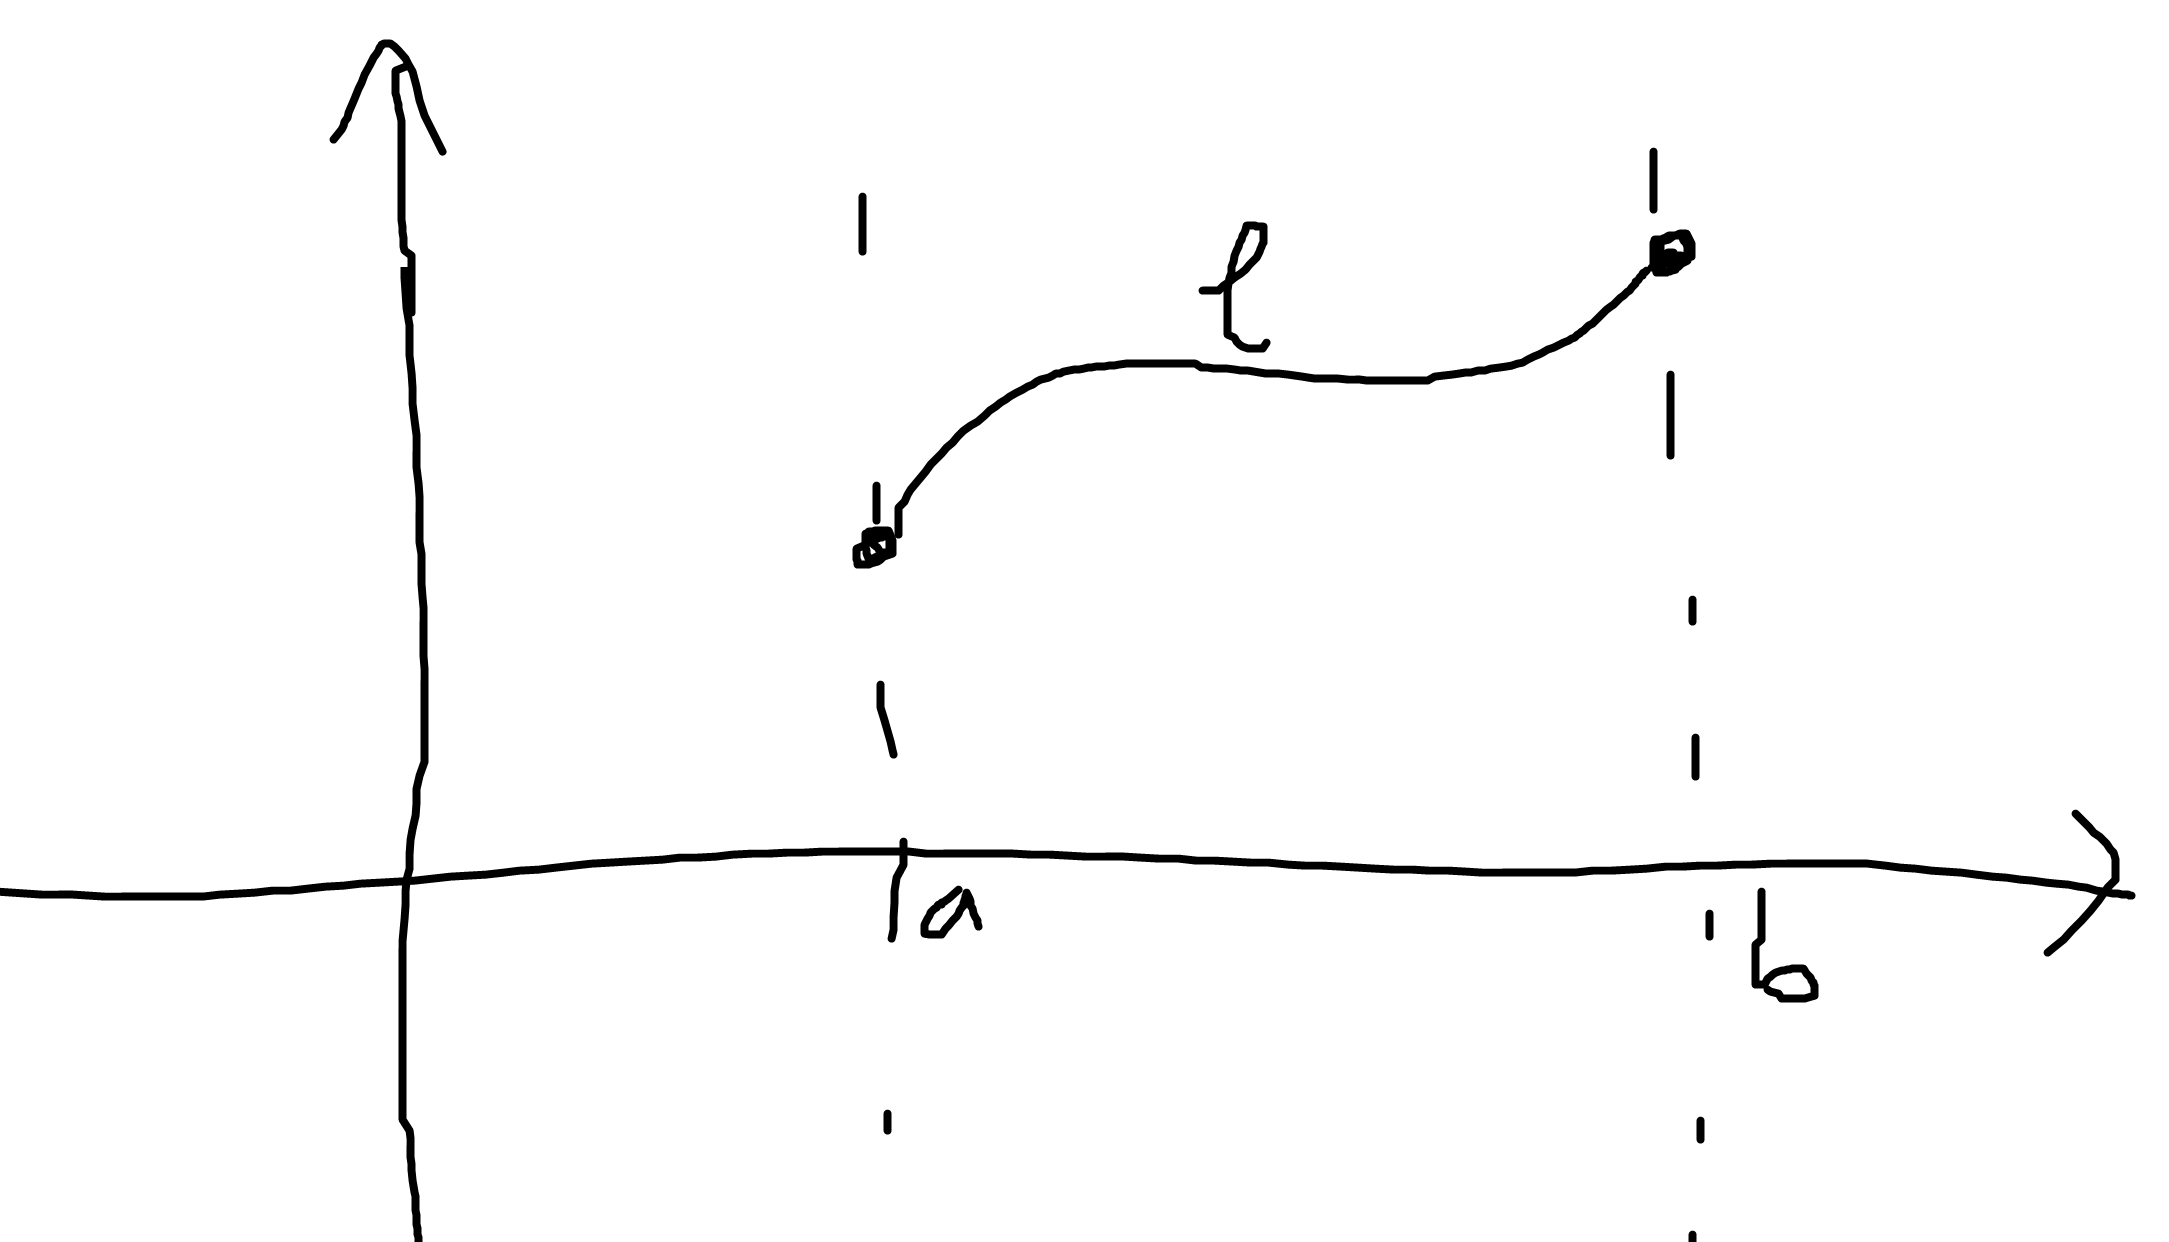
\includegraphics[height=3cm]{kepek/11.png}
			\caption{}
		\end{figure}
		\vspace{-6mm}
		\[ l=\int_a^b\sqrt{1+(f'(x))^2}\,dx \]
	\end{note}
	\begin{example}
		\[ f(x):=\frac{2(x-1)^{\frac{3}{2}}}{3};\quad x\in[2,5] \]
		Megoldás:
		\[ f'(x)=\frac{2}{3}\cdot\frac{3}{2}\cdot(x-1)^\frac{1}{2}=\sqrt{x-1} \]
		\[ \Rightarrow\quad l=\int_2^5\sqrt{1+x-1}\,dx=\int_2^5\sqrt{x}\,dx=\left[\frac{x^\frac{3}{2}}{\frac{3}{2}}\right]_2^5=\frac{2}{3}\left(5\sqrt{5}-2\sqrt{2}\right) \]
	\end{example}
	\begin{exercise}
		\[ f(x):=\sqrt{x};\quad x\in[1,2] \]
		Mekkora ívének hossza 1 és 2 között?
		\begin{figure}[H]
			\centering
			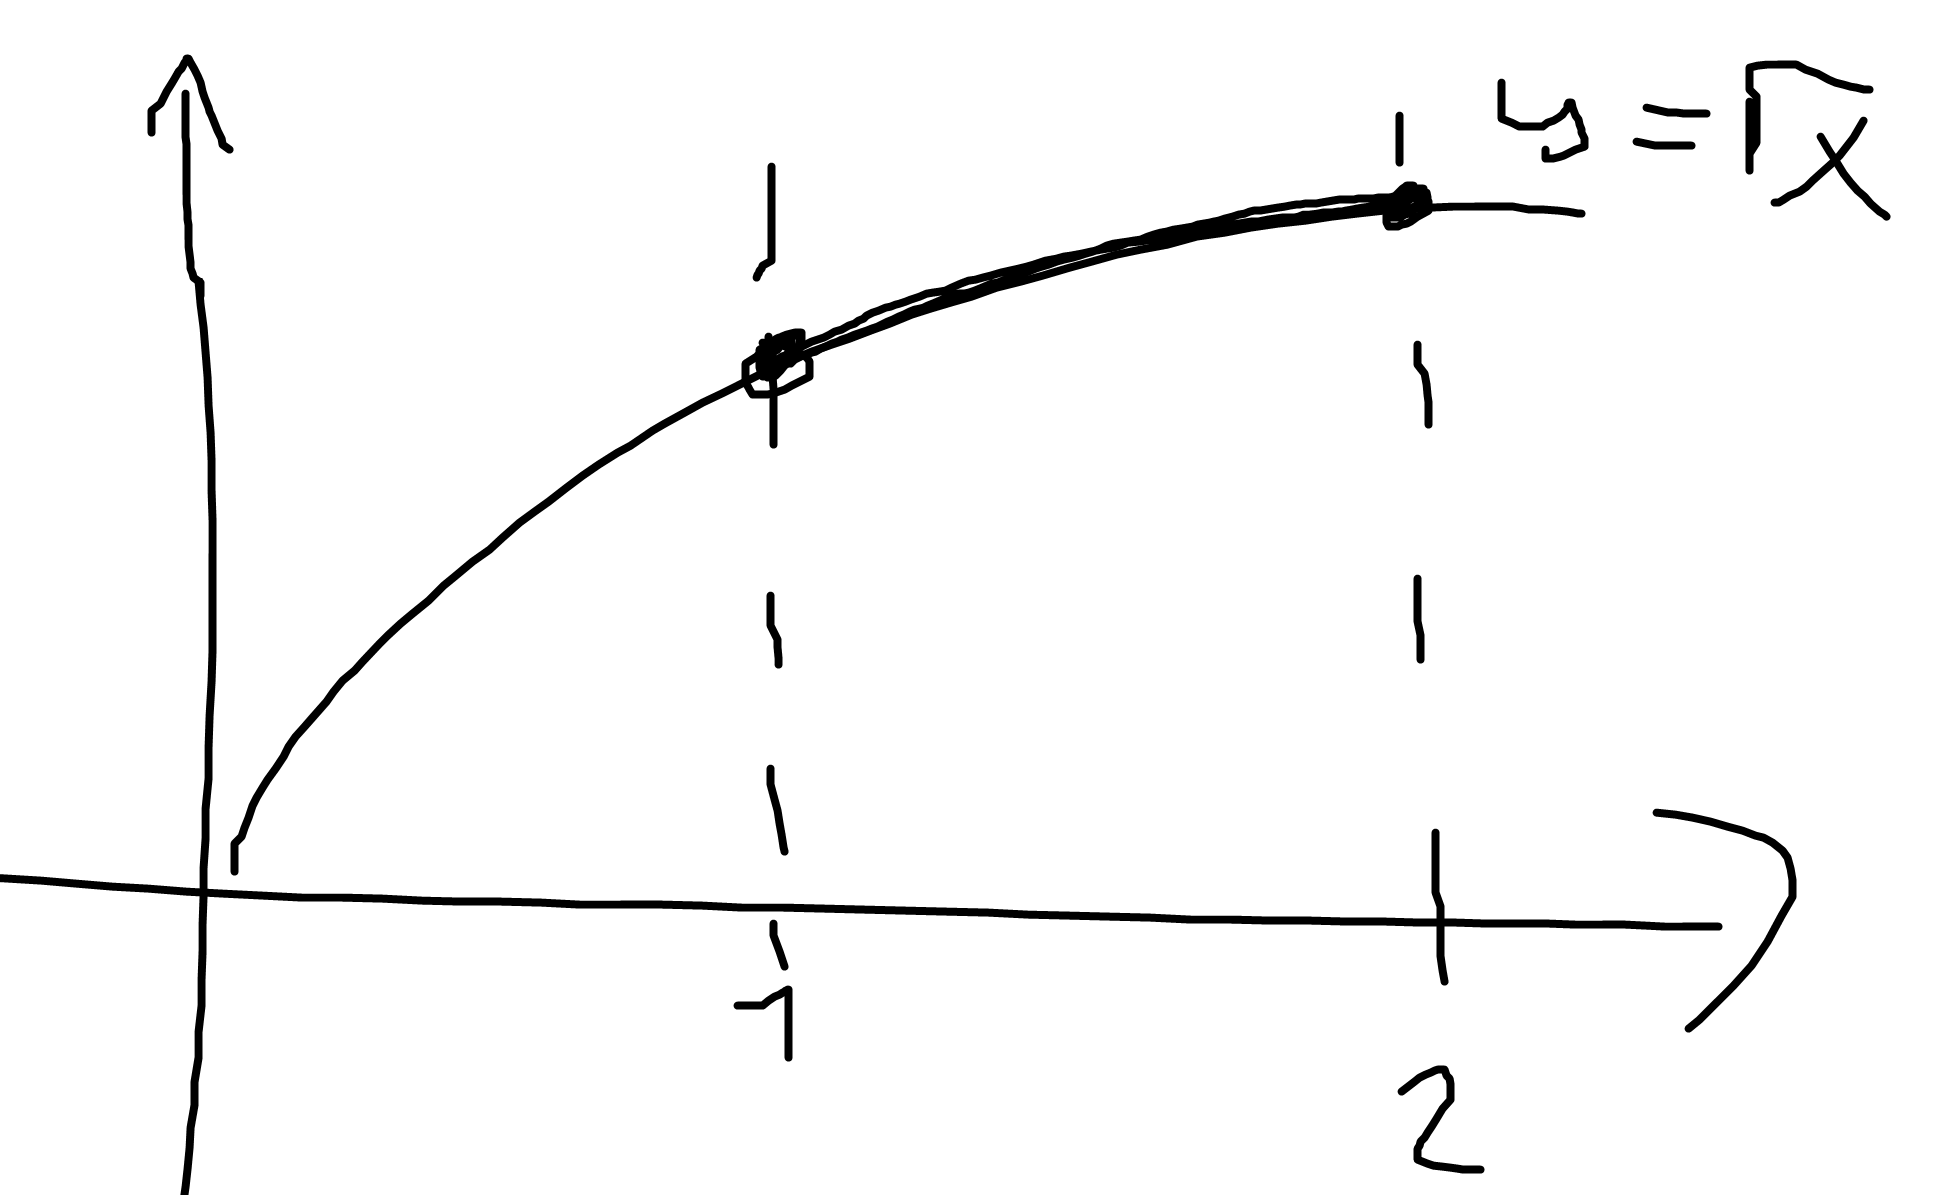
\includegraphics[height=3cm]{kepek/12.png}
			\caption{}
		\end{figure}
		Megoldás:
		\[ \Rightarrow\quad l=\int_1^2\sqrt{1+\left[(\sqrt{x}')\right]^2}\,dx=\int_1^2\sqrt{1+\left(\frac{1}{2\sqrt{x}}\right)^2}\,dx=\int_1^2\sqrt{1+\frac{1}{4x}}\,dx=\frac{1}{2}\cdot\int_1^2\sqrt{\frac{4x+1}{x}}\,dx= \]
		Vezessünk be egy új változót:
		\[ t:=\sqrt{\frac{4x+1}{x}},\quad x=\frac{1}{t^2-4},\quad dx=-\frac{2t}{(t^2-4)^2}\,dt\]
		Megállapítható, hogy 
		\[ x=1\quad \Rightarrow\quad t=\sqrt{5} \]
		\[ x=2\quad \Rightarrow\quad t=\frac{3}{\sqrt{2}} \]
		Visszatérve:
		\[ =-\frac{1}{2}\cdot\int_{\sqrt{5}}^{\frac{3}{\sqrt{2}}}t\left(\frac{2t}{(t^2-4)^2}\right)\,dt\quad \overset{\int_a^bf=-\int_b^af}{=}\quad \int_{\frac{3}{\sqrt{2}}}^{\sqrt{5}}\frac{t^2}{(t-2)^2(t+2)^2}\,dt=\]
		\[=\int_{\frac{3}{\sqrt{2}}}^{\sqrt{5}}\left(\frac{A}{t-2}+\frac{B}{(t-2)^2}+\frac{C}{t+2}+\frac{D}{(t+2)^2}\right)\,dt=\]
		\textit{A feladat befejezése:} Határozzuk meg $A,B,C,D\in\R$-t.
		\begin{align*}
			t^2\quad &=\quad A(t-2)(t+2)^2+B(t+2)^2+C(t+2)(t-2)^2+D(t-2)^2=\\
					 &=\quad A(t^2-4)(t+2)+B(t+2)^2+C(t^2-4)(t-2)+D(t-2)^2=\\
					 &=\quad A(t^3+2t^2-4t-8)+B(t^2+4t+4)+C(t^3-2t^2-4t+8)+D(t^2-4t+4)=\\
					 &=\quad (A+C)t^3+(2A+B-2C+D)t^2+(-4A+4B-4C-4D)t+(-8A+4B+8C+4D)
		\end{align*}
		\textit{Értékadással} könnyen megadható pár konstans.
		\begin{align*}
		t=-2\quad \Rightarrow&\quad 4=16D\quad \Leftrightarrow\quad D=\frac{1}{4}\\
		t=2\quad \Rightarrow &\quad 4=16B\quad \Leftrightarrow\quad B=\frac{1}{4}
		\end{align*}
		Így könnyebben számolható a többi konstans \textit{egyenlő együtthatók} módszerével.
		\begin{align*}
			t^3 \quad \text{együtthatója:}\quad 0&=A+C\\
			t^2 \quad \text{együtthatója:}\quad 
												1&=2A+\frac{1}{4}-2C+\frac{1}{4}\\
											   \frac{1}{4}&=A-C\\
			t^1 \quad \text{együtthatója:}\quad 0&=-4A+1-4C-1\\
												0&=-A-C\\
			t^0 \quad \text{együtthatója:}\quad 0&=-8A+1+8C+1\\
												1&=-4A+4C
		\end{align*}
		Ez alapján megállapítható hogy $C=-\frac{1}{8}$ és $A=\frac{1}{8}$. Visszatérve:
		\[=-\frac{1}{8}\cdot\int_{\frac{3}{\sqrt{2}}}^{\sqrt{5}}\frac{1}{t-2}\,dt+\frac{1}{4}\cdot\int_{\frac{3}{\sqrt{2}}}^{\sqrt{5}}\frac{1}{(t-2)^2}\,dt+\frac{1}{8}\cdot\int_{\frac{3}{\sqrt{2}}}^{\sqrt{5}}\frac{1}{t+2}\,dt+\frac{1}{4}\cdot\int_{\frac{3}{\sqrt{2}}}^{\sqrt{5}}\frac{1	}{(t+2)^2}\,dt=\]
		\[= \frac{1}{8}\left(-\Big[\ln(t-2)\Big]^{\sqrt{5}}_{\frac{3}{\sqrt{2}}}+2\left[-\frac{1}{1-2}\right]^{\sqrt{5}}_{\frac{3}{\sqrt{2}}}+\Big[\ln(t+2)\Big]^{\sqrt{5}}_{\frac{3}{\sqrt{2}}}+2\left[-\frac{1}{t+2}\right]^{\sqrt{5}}_{\frac{3}{\sqrt{2}}} \right)\]
		Megállapítható, hogy a területe létezik.~~~:)
	\end{exercise}
	\begin{note}
		Megállapítható, hogy $x^2$-te visszavezethető a $\sqrt{x}$ függvény.
		
		\begin{figure}[H]
			\centering
			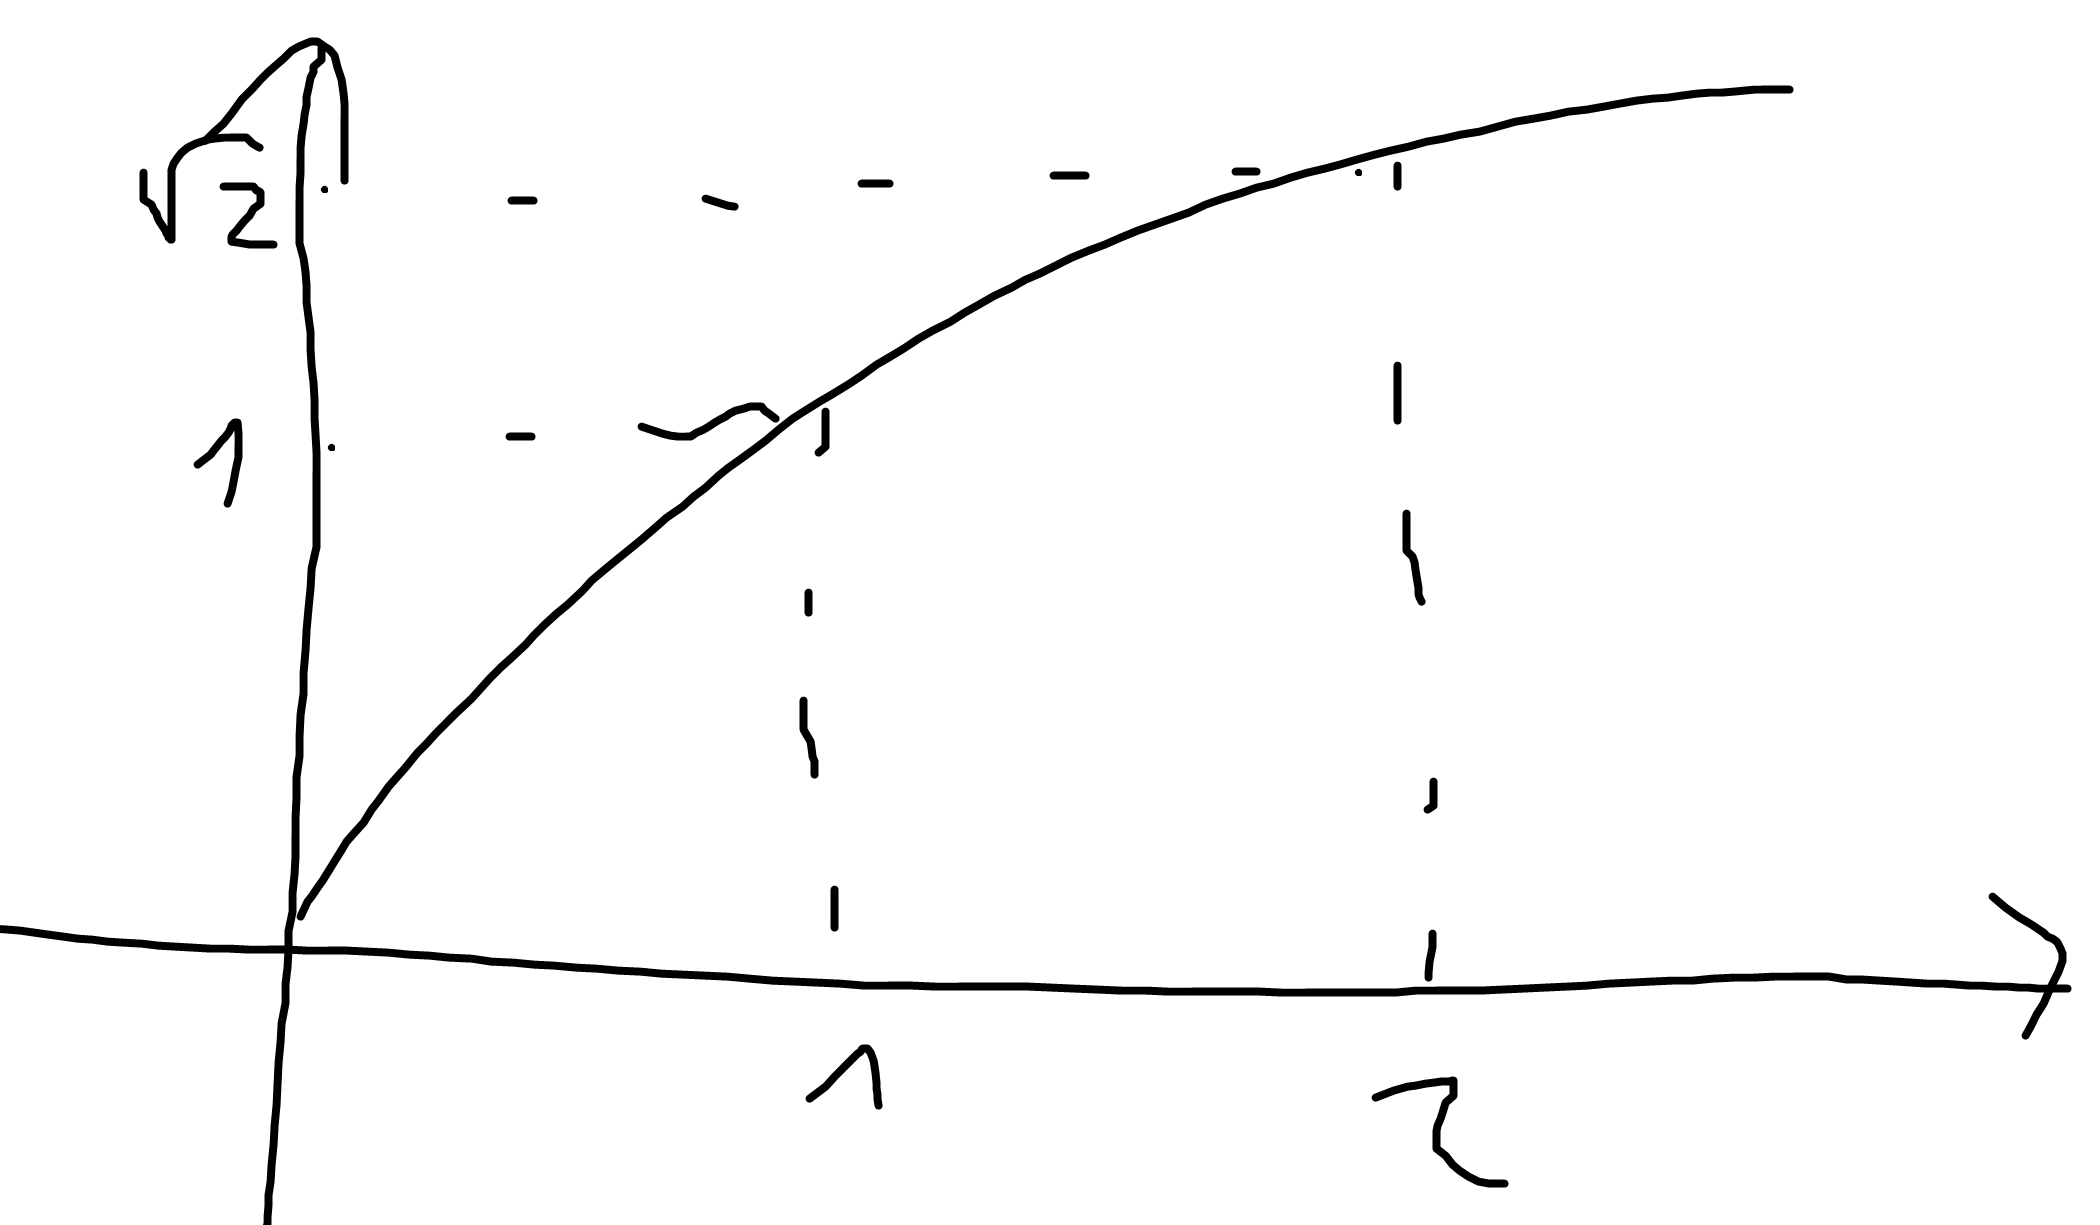
\includegraphics[height=3cm]{kepek/13.png}\quad \quad \quad 
			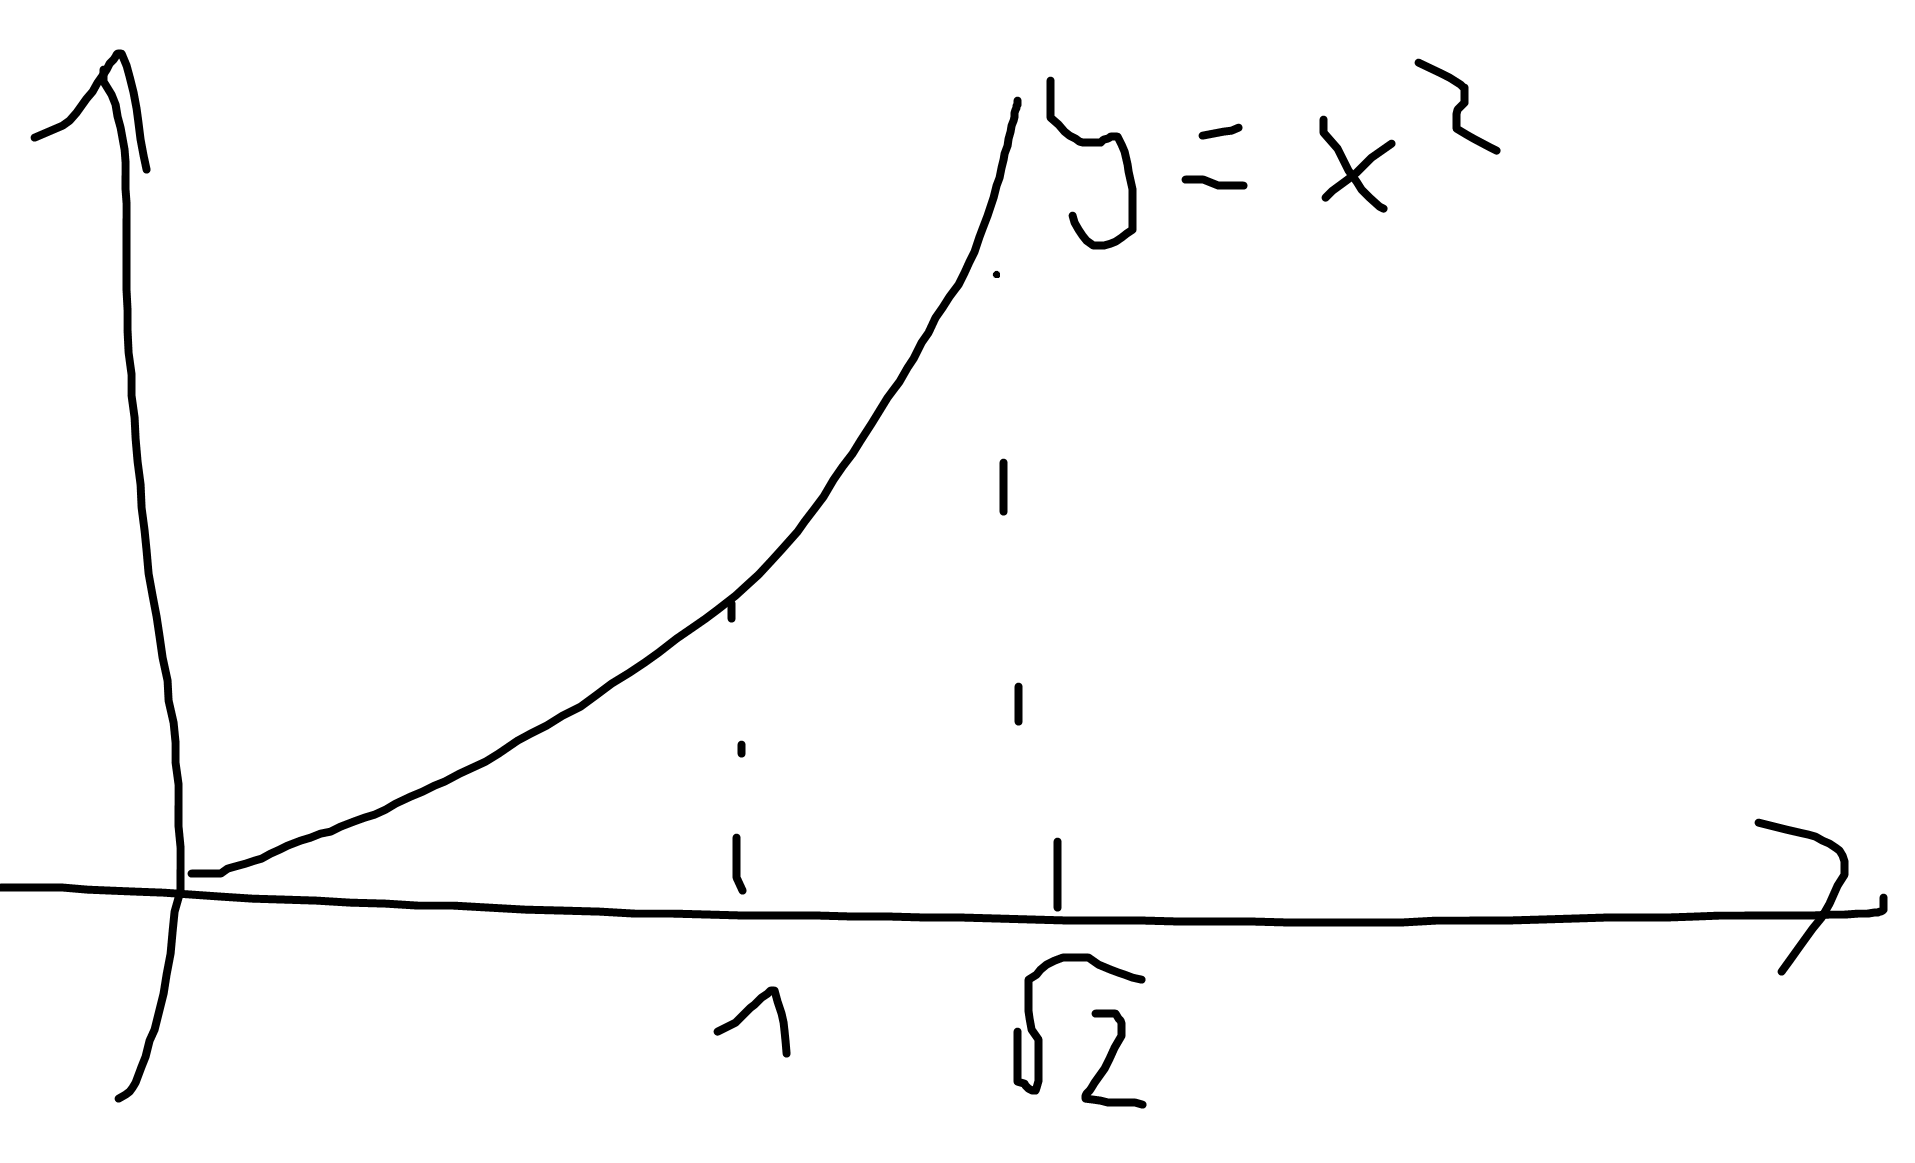
\includegraphics[height=3cm]{kepek/14.png}
			\caption{}
		\end{figure}
		\[ \Rightarrow\quad l=\int_1^{\sqrt{2}}\sqrt{1+4x^2}\,dx= \]
		Befejezése házi, javallott a $2x=\sh t$ helyettesítés.
	\end{note}
	\subsubsection{Forgástestek térfogata és felszíne}
	\begin{revision}
		\begin{figure}[H]
			\centering
			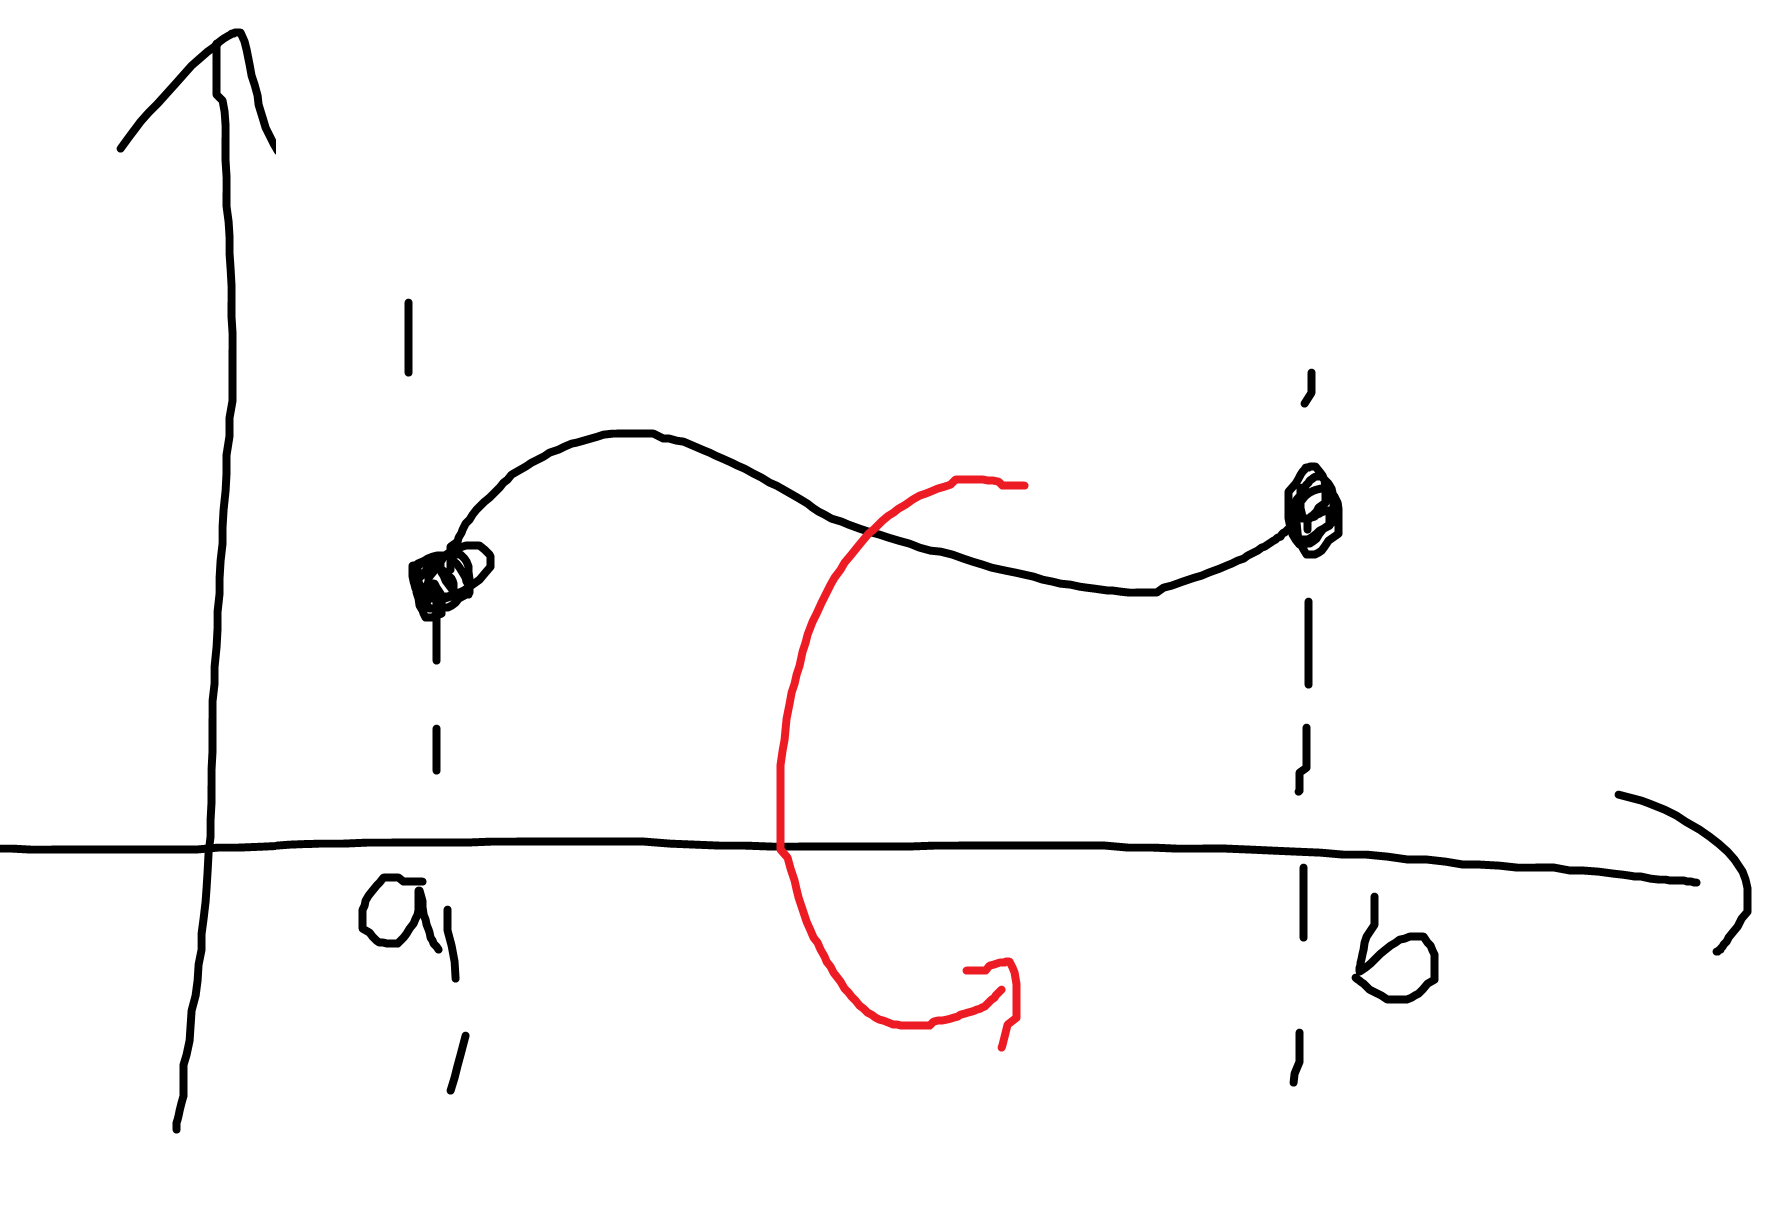
\includegraphics[height=3cm]{kepek/15pre.png}$\quad \quad \quad $
			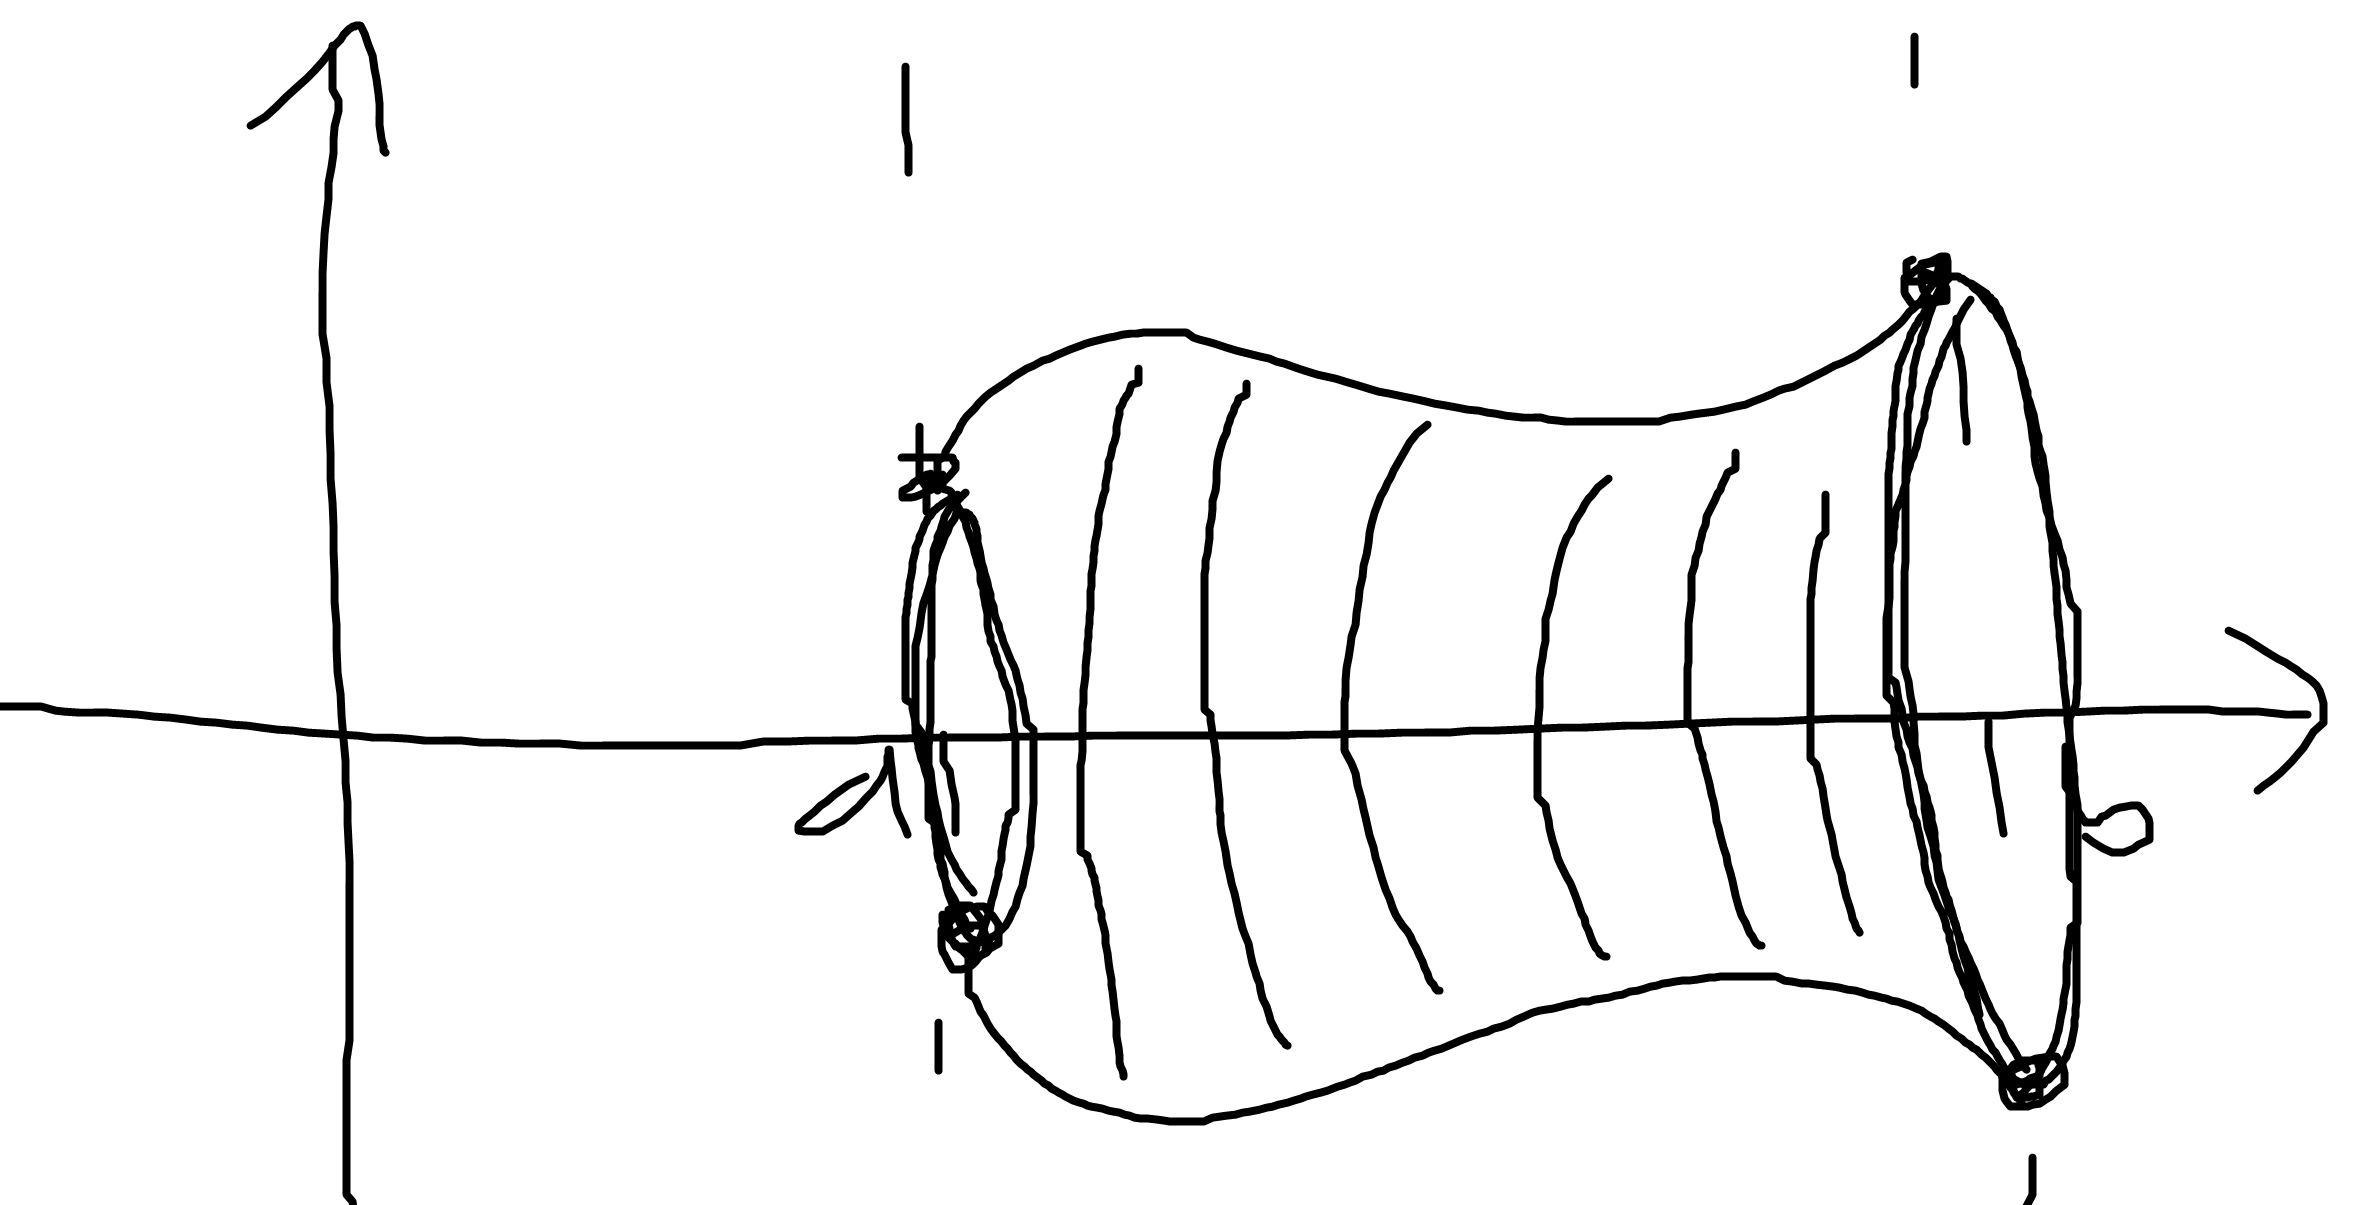
\includegraphics[height=3cm]{kepek/15.png}
			\caption{}\label{rotation}
		\end{figure}
		Ha a \ref{rotation}. ábrán lévő példát megforgatjuk az $x$ tengely körül, egy testet kapunk, melynek térfogatát számolhatjuk határozott integrállal.
		\[ V=\pi\int_a^bf^2(x)\,dx\quad (f\in\R[a,b]) \]
		\[ \mathcal{F}=2\pi\int_a^bf(x)\cdot\sqrt{1+(f'(x))^2}\,dx\quad (f\in C^1[a,b]) \]
		Ahol $V$ a térfogat (\textit{volume}) és $\mathcal{F}$ a felület.
	\end{revision}
	\begin{example} Határozzuk meg $f$ függvény $x$ tengely körüli forgástestének térfogatát ($V$), felületét ($\mathcal{F}$), és $f$ függvény alatti területét ($T$).
		\[ f(x):=\sin x\quad x\in[0,\pi]\]
		\begin{figure}[H]
			\centering
			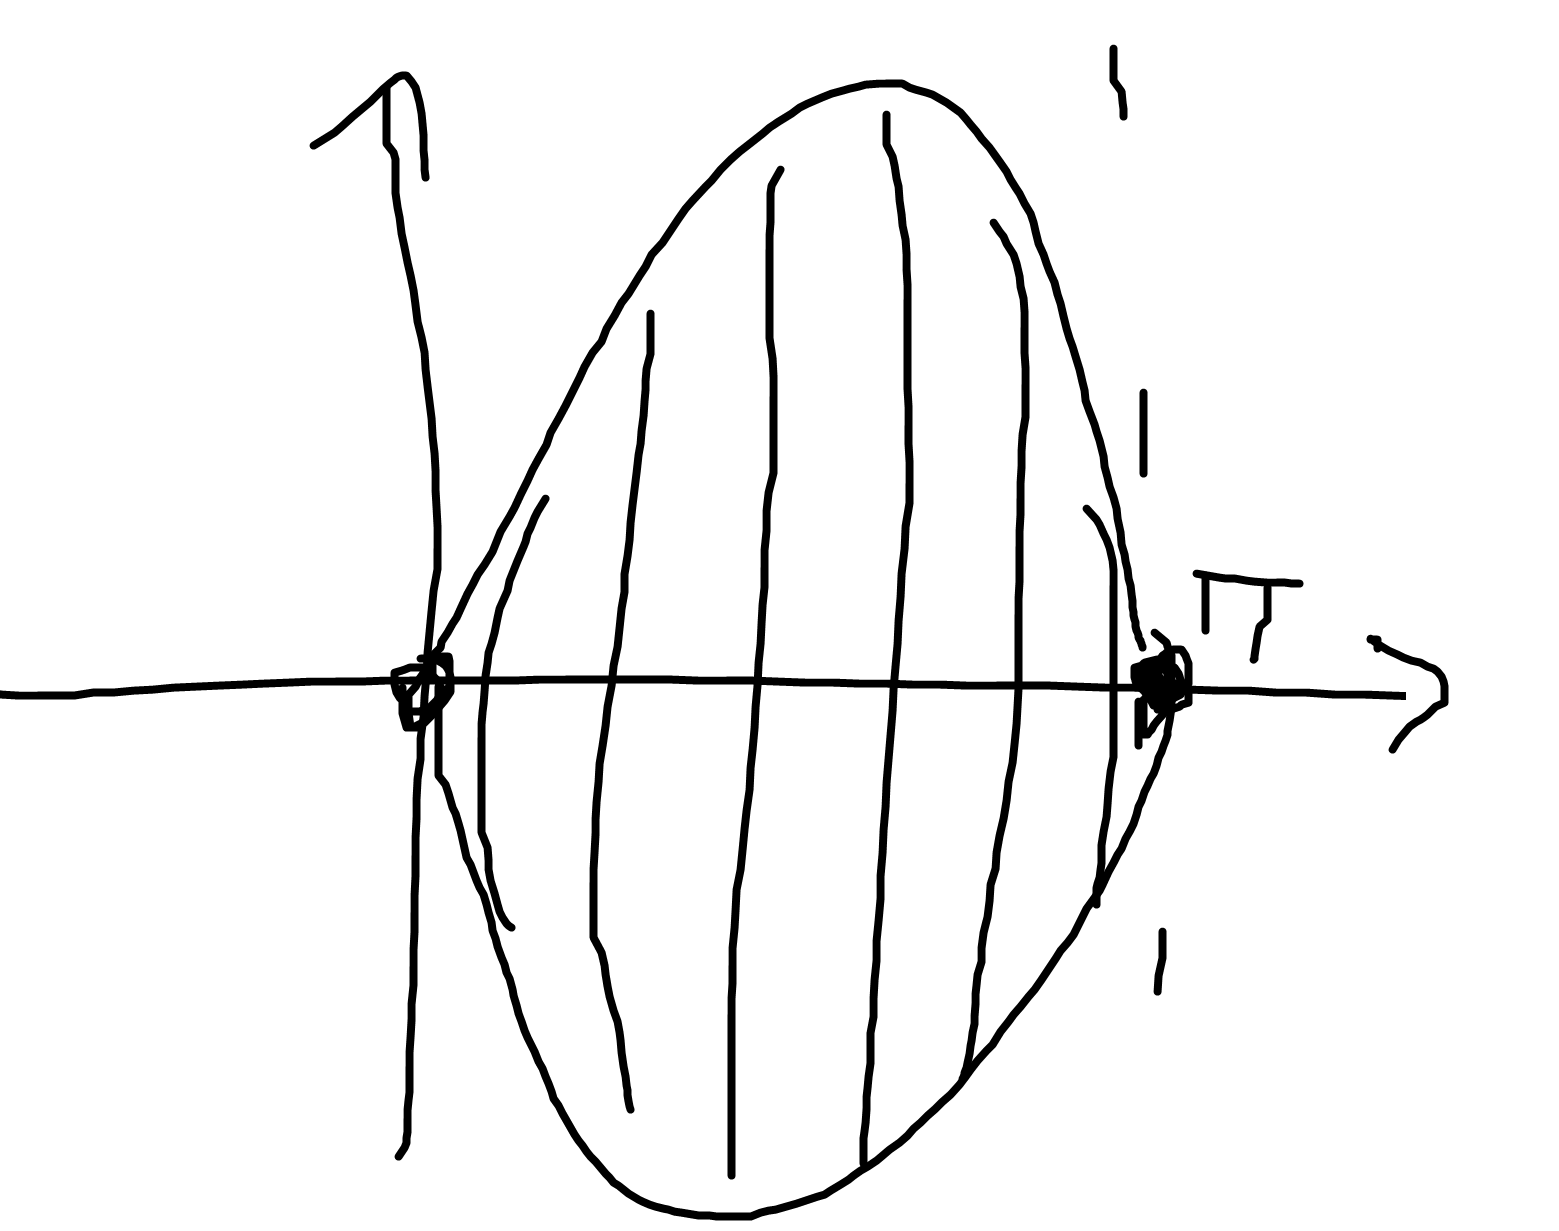
\includegraphics[height=3cm]{kepek/16.png}
			\caption{}
		\end{figure}
		\vspace{-6mm}
		\[ T=\int_0^\pi\sin x\,dx=\left[-\cos x\right]_0^\pi=1+\cos 0=2 \]
		\[ V=\pi\int_0^\pi\sin^2x\,dx=\frac{\pi}{2}\cdot\left[x-\frac{\sin2x}{2}\right]_0^\pi=\frac{\pi}{2}\cdot\left[\pi-\frac{\sin2\pi}{2}-0\right]=\frac{\pi^2}{2} \]
		Folytatván
		\[ \mathcal{F}=2\pi\cdot\int_0^\pi \sin x\cdot\sqrt{ 1+\cos^2x}\,dx= \]
		Vezessünk be egy új változót.
		\[ \sh t:=\cos x,\quad -\sin x\,dx=\ch t\,dt \]
		Visszatérve:
		\[ 2\pi\cdot\int \sin x\cdot\sqrt{ 1+\cos^2x}\,dx=2\pi\cdot\int\sqrt{1+\sh^2t}\cdot(-\ch t)\,dt \]
		\[ x=0\quad \Rightarrow\quad 1=\sh t\quad \Rightarrow\quad t=\arsh 1=\ln(\sqrt{2}+1) \]
		\[ x=\pi\quad \Rightarrow\quad -1=\sh t\quad \Rightarrow\quad t=\arsh (-1)=\ln(\sqrt{2}-1) \]
		\[ \arsh x=\ln(x+\sqrt{1+x^2}) \]
		Befejetése hf.
	\end{example}
	\begin{exercise}
		\[ f(x)=2\cdot\sqrt{1-x^2}\quad x\in[-1,1] \]
		Forgástest $V, \mathcal{F}=?$
		
		\[ y^2=2\sqrt{1-x^2}\quad \Rightarrow\quad \frac{y^2}{4}+x^2=1 \]
		\[ \frac{x^2}{a^2}+\frac{y^2}{b^2}=1 \]
	\end{exercise}
\end{document}